\documentclass[10pt,twocolumn,a4paper]{article}

\usepackage[utf8]{inputenc}
\usepackage[top=0.65in,bottom=0.68in,left=0.65in,right=0.65in,headheight=13pt,headsep=12pt,columnsep=0.22in]{geometry}
\usepackage{amsmath,amssymb}
\usepackage{graphicx}
\graphicspath{{images/}{report/images/}{../report/images/}}
\usepackage{booktabs}
\usepackage{tabularx}
\usepackage{xurl}
\usepackage{hyperref}
\usepackage{xcolor}
\usepackage{fancyhdr}
\usepackage{caption}
\usepackage{subcaption}
\usepackage{float}
\usepackage{enumitem}
\usepackage{microtype}
\usepackage{titlesec}

% Compact section headings to optimize space and ensure strict <= 10 page compliance
\titlespacing*{\section}{0pt}{7pt plus 1.5pt minus 1.5pt}{3pt plus 1pt minus 1pt}
\titlespacing*{\subsection}{0pt}{5pt plus 1pt minus 1pt}{2pt plus 0.5pt minus 0.5pt}
\titlespacing*{\subsubsection}{0pt}{3.5pt plus 1pt minus 0.5pt}{1.5pt plus 0.5pt minus 0.5pt}

\hypersetup{
    colorlinks=true,
    linkcolor=blue!70!black,
    citecolor=green!50!black,
    urlcolor=blue!70!black
}

\newcommand{\githubrepo}{https://github.com/CL3-410/individual-project-Rajkjain03/blob/phase-3/report/}

\pagestyle{fancy}
\fancyhf{}
\fancyhead[L]{\small\textsf{Language Models and Agents (Monsoon 2026) --- Consolidated 3-Phase Report}}
\fancyhead[R]{\small\textsf{Raj k jain (Roll No. 2025201036)}}
\fancyfoot[C]{\small\thepage}
\renewcommand{\headrulewidth}{0.4pt}
\renewcommand{\footrulewidth}{0pt}

\fancypagestyle{plain}{
  \fancyhf{}
  \fancyfoot[C]{\small\thepage}
  \renewcommand{\headrulewidth}{0pt}
}

\title{\vspace{-1.2em}\textbf{\Large From-Scratch Monolingual Transformer Language Models for Hindi and Nepali: Pretraining, Diagnostic Attention Dynamics, Reasoning Finetuning, and Positional Ablation}\vspace{-0.5em}}
\author{\textbf{Raj k jain} \quad\textbullet\quad Roll No.: \texttt{2025201036} \quad\textbullet\quad \texttt{raj.jain@students.iiit.ac.in} \\
\small International Institute of Information Technology, Hyderabad (IIIT-H)\vspace{-1.0em}}
\date{\vspace{-0.6em}\small September 2026}

\begin{document}

\twocolumn[
  \begin{@twocolumnfalse}
    \maketitle
    \begin{abstract}
    \small
    This report provides a unified, first-principles scientific account of building, pretraining, evaluating, analyzing, and finetuning two completely independent decoder-only Transformer language models for two Indian languages written in Devanagari: Hindi (\textbf{Model H}, higher-resource tier) and Nepali (\textbf{Model L}, lower-resource tier). Neither pretrained models, tokenizers, nor third-party Transformer abstractions were utilized. In \textbf{Phase 1}, monolingual corpora exceeding 600M tokens per language were curated, cleaned, and partitioned into SQLite databases, followed by training custom SentencePiece BPE tokenizers from scratch (32,000 vocab for Hindi; 16,000 vocab for Nepali), revealing an inverse relationship between subword fertility and downstream vocabulary efficiency. In \textbf{Phase 2}, custom 6-layer, 8-head, 512-dimension decoder-only Transformers equipped with Rotary Position Embeddings (RoPE), pre-norm RMSNorm, SwiGLU feed-forward networks, and student-implemented causal masking were pretrained under optimal Chinchilla compute budgets using AdamW and cosine scheduling. Comprehensive evaluations established a crucial divergence: while Nepali achieved lower cross-entropy loss (3.63 vs. 4.02) and perplexity (37.71 vs. 55.49), Hindi exhibited substantially stronger sentential generation coherence (BLEU-4 of 3.51 vs. 0.00; chrF of 9.19 vs. 4.43) owing to severe train-val generalization gaps in Hindi and morphological predictability in Nepali. To fulfill evaluation feedback, exhaustive attention diagnostics were conducted across \textbf{all 48 heads per model}, establishing an explicit Cartesian coordinate framework ($X$: Key context token, $Y$: Query attending token) and identifying a monotonic expansion of attention span alongside the spontaneous emergence of terminal attention sinks. In \textbf{Phase 3}, deterministic synthetic comparative- and transitive-reasoning datasets with strict leakage controls (20\% held-out entity names; 100\% test-only attribute) were constructed, and supervised finetuning with masked-prompt loss yielded dramatic accuracy gains (+35.75\% in Hindi; +24.00\% in Nepali) while actively dismantling pathological attention sinks. Finally, an \textbf{Ablation Study} retrained the 36.84M parameter Hindi model with positional encodings completely excised, mathematically and empirically proving how self-attention degenerates into word-order permutation invariance, catastrophic autoregressive loops (repetition surges to 71.6\%), and a 47-fold perplexity explosion.
    \end{abstract}
    \vspace{0.8em}
  \end{@twocolumnfalse}
]

\section{Introduction and Architecture Formulation}

Modern autoregressive language modeling predominantly relies on the decoder-only Transformer architecture. While large multilingual models dominate production settings, constructing monolingual models from first principles for non-English languages provides deep insights into tokenization fertility, linguistic structure, resource constraints, and attention specialization.

\subsection{Project Constraints and Compliance}
In strict adherence to course specifications:
\begin{enumerate}[noitemsep,leftmargin=*]
    \item \textbf{No Pretrained Weights or Tokenizers:} No HuggingFace model abstractions, pretrained tokenizers, or external weights were utilized.
    \item \textbf{Zero Cross-Language Leakage:} Model H and Model L share zero training data, tokenizers, vocabularies, or checkpoints.
    \item \textbf{From-Scratch Primitives:} Token embeddings, Rotary Position Embeddings (RoPE), multi-head causal attention, SwiGLU FFNs, and causal masking were implemented directly via primitive PyTorch modules (\texttt{nn.Linear}, \texttt{nn.Embedding}, \texttt{nn.Parameter}).
    \item \textbf{Resumability:} Every training run supports deterministic resumption saving model weights, AdamW optimizer states, cosine scheduler states, and global step counts.
\end{enumerate}

\begin{table}[t]
\centering
\footnotesize
\setlength{\tabcolsep}{2.5pt}
\caption{System Specifications and Hyperparameters at a Glance}
\label{tab:system_overview}
\begin{tabularx}{\columnwidth}{@{}>{\raggedright\arraybackslash}p{2.5cm}>{\raggedright\arraybackslash}X>{\raggedright\arraybackslash}X@{}}
\toprule
\textbf{Hyperparameter} & \textbf{Model H (Hindi)} & \textbf{Model L (Nepali)} \\
\midrule
Language Tier & Higher-Resource & Lower-Resource \\
Script & Devanagari & Devanagari \\
Vocabulary Size & 32,000 tokens & 16,000 tokens \\
Context Length ($T$) & 512 tokens & 512 tokens \\
Layers ($N$) / Heads ($h$) & 6 layers / 8 heads & 6 layers / 8 heads \\
Model Dim ($d_{\text{model}}$) / $d_k$ & 512 / 64 & 512 / 64 \\
FFN Dim ($d_{\text{ff}}$) & 2,048 (SwiGLU) & 2,048 (SwiGLU) \\
Positional Embedding & RoPE ($\theta=10^4$) & RoPE ($\theta=10^4$) \\
Normalization & RMSNorm ($\epsilon=10^{-6}$) & RMSNorm ($\epsilon=10^{-6}$) \\
Weight Tying & In/Out Tied & In/Out Tied \\
\textbf{Trainable Params} & \textbf{36,837,888} & \textbf{28,645,888} \\
Training Compute & RTX 3050 (4GB) & RTX 3050 (4GB) \\
\bottomrule
\end{tabularx}
\end{table}

\subsection{Mathematical Architecture Formulation}
The implemented architecture is a causal decoder-only Transformer:

\subsubsection{Rotary Position Embeddings (RoPE)}
Rather than additive absolute sinusoidal encodings, Rotary Position Embeddings were incorporated directly into the query-key dot product. For position $t \in [0, T-1]$, the 2D rotation matrix for coordinate slice $i \in [0, d_k/2 - 1]$ is:
\begin{equation}
R_{\theta_i, t} = \begin{pmatrix} \cos(t\theta_i) & -\sin(t\theta_i) \\ \sin(t\theta_i) & \cos(t\theta_i) \end{pmatrix}, \quad \theta_i = 10000^{-2i/d_k}
\end{equation}
When queries $q_t$ and keys $k_s$ are rotated, their inner product satisfies $(R_t q)^T (R_s k) = q^T R_{s - t} k$, preserving relative positional offset invariant under absolute translation.

\subsubsection{Multi-Head Attention and Causal Masking}
For hidden representation $H \in \mathbb{R}^{B \times T \times d_{\text{model}}}$, linear projections yield queries, keys, and values:
\begin{equation}
Q = HW_Q, \quad K = HW_K, \quad V = HW_V
\end{equation}
Tensors are reshaped to $(B, h, T, d_k)$. The attention matrix $A \in \mathbb{R}^{T \times T}$ is computed with a strictly lower-triangular causal mask $M$:
\begin{equation}
A = \text{softmax}\left( \frac{R(Q) R(K)^T}{\sqrt{d_k}} + M \right)
\end{equation}
where $M_{ij} = 0$ for $j \le i$, and $M_{ij} = -\infty$ for $j > i$.
The scaling factor $1/\sqrt{d_k} = 1/\sqrt{64} = 0.125$ counteracts dot-product variance growth that pushes softmax into vanishing gradient regimes.

\paragraph{Empirical Causal Mask Verification:}
To rigorously verify zero future information leakage, sequence $A$ was passed through Model H, recording output logits at position $t=2$. Sequence $B$ was created by modifying a token at $t=5$. The observed difference at $t=2$ was:
\begin{equation}
\max |\text{Logits}_A[2, :] - \text{Logits}_B[2, :] | = \mathbf{0.000000}
\end{equation}
while position $t=5$ exhibited a substantial divergence of 6.7968. This proves that autoregressive masking is strictly enforced.

\subsubsection{Transformer Block: Pre-Norm RMSNorm and SwiGLU}
Each layer applies Pre-Norm Root Mean Square Normalization:
\begin{equation}
\text{RMSNorm}(x) = \frac{x}{\sqrt{\frac{1}{d}\sum_{i=1}^d x_i^2 + \epsilon}} \odot \gamma
\end{equation}
Pre-norm maintains a clean residual stream, preventing gradient attenuation. The Feed-Forward Network employs the SwiGLU activation function:
\begin{equation}
\text{FFN}_{\text{SwiGLU}}(x) = \left( \text{SiLU}(xW_1) \otimes xW_3 \right) W_2
\end{equation}
where $W_1, W_3 \in \mathbb{R}^{d \times d_{\text{ff}}}$ and $W_2 \in \mathbb{R}^{d_{\text{ff}} \times d}$ with $d_{\text{ff}} = \frac{2}{3}(4d) = 2048$.

\subsubsection{Weight Tying}
The output linear unembedding matrix is tied directly to the input token embedding table ($W_{\text{out}} = W_{\text{emb}}^T$). This saved 16.38M parameters in Hindi ($32000 \times 512$) and 8.19M parameters in Nepali ($16000 \times 512$).

\section{Phase 1: Corpus Curation and Tokenization}

\subsection{Language Selection Justification}
\textbf{Hindi (Model H, Higher-Resource):} Spoken by over 600 million individuals, Hindi has extensive digital web presence and rich standardized text in Devanagari. The AI4Bharat Sangraha corpus provided hundreds of millions of clean tokens, readily supporting our $>600\text{M}$ token target.
\textbf{Nepali (Model L, Lower-Resource):} An officially scheduled Indian language prominent in Sikkim and West Bengal, Nepali also uses Devanagari but features distinct agglutinative morphology, complex case-marking enclitics, and lower digital corpus availability.

\subsection{Dataset Ingestion and Preprocessing Pipeline}
The data engineering pipeline was designed for memory safety and resumption. Raw streams were ingested into structured SQLite databases (\texttt{hindi\_state.db} and \texttt{nepali\_state.db}) indexed by MD5 document hashes:
\begin{enumerate}[noitemsep,leftmargin=*]
    \item \textbf{Public Corpus Streaming:} Streamed in chunks from verified splits of the AI4Bharat Sangraha corpus to prevent RAM crashes.
    \item \textbf{Manual Data Collection:} Scanned regional literature and public-domain books were OCR'd using Tesseract (\texttt{tesseract-ocr-hin}, \texttt{tesseract-ocr-nep}) with custom bounding-box cleanup.
    \item \textbf{Text Normalization:} NFKC Unicode normalization, removal of broken codepoint sequences, Devanagari character verification, and filtering of non-linguistic web boilerplate.
    \item \textbf{Splits:} Deterministically split into 90\% train, 5\% validation, and 5\% test partitions.
\end{enumerate}

\begin{table}[t]
\centering
\footnotesize
\setlength{\tabcolsep}{2.5pt}
\caption{Phase 1 Corpus Statistics and Token Accounting}
\label{tab:phase1_stats}
\begin{tabularx}{\columnwidth}{@{}>{\raggedright\arraybackslash}Xrr@{}}
\toprule
\textbf{Corpus Metric} & \textbf{Hindi (Model H)} & \textbf{Nepali (Model L)} \\
\midrule
Total Documents & 1,323,072 & 1,836,292 \\
Total Tokens (All Splits) & 681,200,436 & 775,992,967 \\
\textbf{Training Tokens} & \textbf{613,059,508} & \textbf{698,466,193} \\
Validation Tokens & 34,070,464 & 38,763,387 \\
Test Tokens & 34,070,464 & 38,763,387 \\
Manual Tokens & 6.78M (1.11\%) & 0.32M (0.05\%) \\
Downloaded Tokens & 606.28M (98.89\%) & 698.14M (99.95\%) \\
Database Size on Disk & 8.0 GB & 11.0 GB \\
\bottomrule
\end{tabularx}
\end{table}

\noindent\textit{Transparent Note on Manual Data Target:} The initial guidelines targeted $\ge 20\%$ manual data. Because achieving optimal pretraining under Chinchilla scaling required exceeding 600M tokens, manual OCR collection represented 1.11\% in Hindi and 0.05\% in Nepali. This trade-off prioritized compute-optimal token volume over manual OCR noise.

\subsection{Tokenizer Training and Fertility Diagnostics}
Independent SentencePiece Byte-Pair Encoding (BPE) tokenizers were trained from scratch on 10 million sample lines per language.
\begin{itemize}[noitemsep,leftmargin=*]
    \item \textbf{Model H (32,000 vocab):} Accommodates Hindi's vast morphological inventory, minimizing subword splitting.
    \item \textbf{Model L (16,000 vocab):} Sized for Nepali's smaller corpus to prevent subword sparsity and unobserved tail tokens.
\end{itemize}

\begin{table}[t]
\centering
\footnotesize
\setlength{\tabcolsep}{3.0pt}
\caption{Tokenizer Quality and Subword Diagnostics}
\label{tab:tokenizer_stats}
\begin{tabularx}{\columnwidth}{@{}>{\raggedright\arraybackslash}Xcc@{}}
\toprule
\textbf{Tokenizer Diagnostic} & \textbf{Hindi Tokenizer} & \textbf{Nepali Tokenizer} \\
\midrule
Algorithm & \multicolumn{2}{c}{SentencePiece BPE} \\
Vocabulary Size & 32,000 tokens & 16,000 tokens \\
Avg. Characters / Token & 4.12 & 4.59 \\
\textbf{Fertility (Tokens/Word)} & \textbf{1.24} & \textbf{1.40} \\
\textbf{Validation UNK Rate} & \textbf{0.0485\%} & \textbf{0.1585\%} \\
\bottomrule
\end{tabularx}
\end{table}

\noindent\textbf{Key Finding:} Nepali exhibits significantly higher fertility (1.40 vs. 1.24 tokens/word) and a $3.27\times$ higher out-of-vocabulary rate (0.1585\% vs. 0.0485\%). This structural fragmentation creates greater cognitive load for Model L, as words are split into smaller particles.

\section{Phase 2: Pretraining Dynamics and Generation Evaluation}

\subsection{Pretraining Protocol and Compute Budget}
Pretraining was conducted using AdamW ($\beta_1=0.9, \beta_2=0.95, \text{weight decay}=0.01$), Cosine Annealing learning rate schedule ($\text{peak}=5\times 10^{-4}, \text{min}=1\times 10^{-5}$), gradient accumulation of 16 steps (effective batch size 64 sequences $\times$ 512 tokens = 32,768 tokens/step), and Automatic Mixed Precision (AMP FP16).
\begin{itemize}[noitemsep,leftmargin=*]
    \item \textbf{Hindi Pretraining:} 18,750 steps $\times$ 32,768 tokens $\approx$ \textbf{614.4M tokens} (1.002 epochs over 613.1M training tokens).
    \item \textbf{Nepali Pretraining:} 21,324 steps $\times$ 32,768 tokens $\approx$ \textbf{698.7M tokens} (1.000 epochs over 698.5M training tokens).
\end{itemize}
Under Chinchilla scaling laws ($D \approx 20N$), a 30M parameter model is compute-optimal at $\sim 600\text{M}$ tokens. Our training runs were mathematically scaled to hit this exact compute budget.

\begin{figure}[t]
\centering
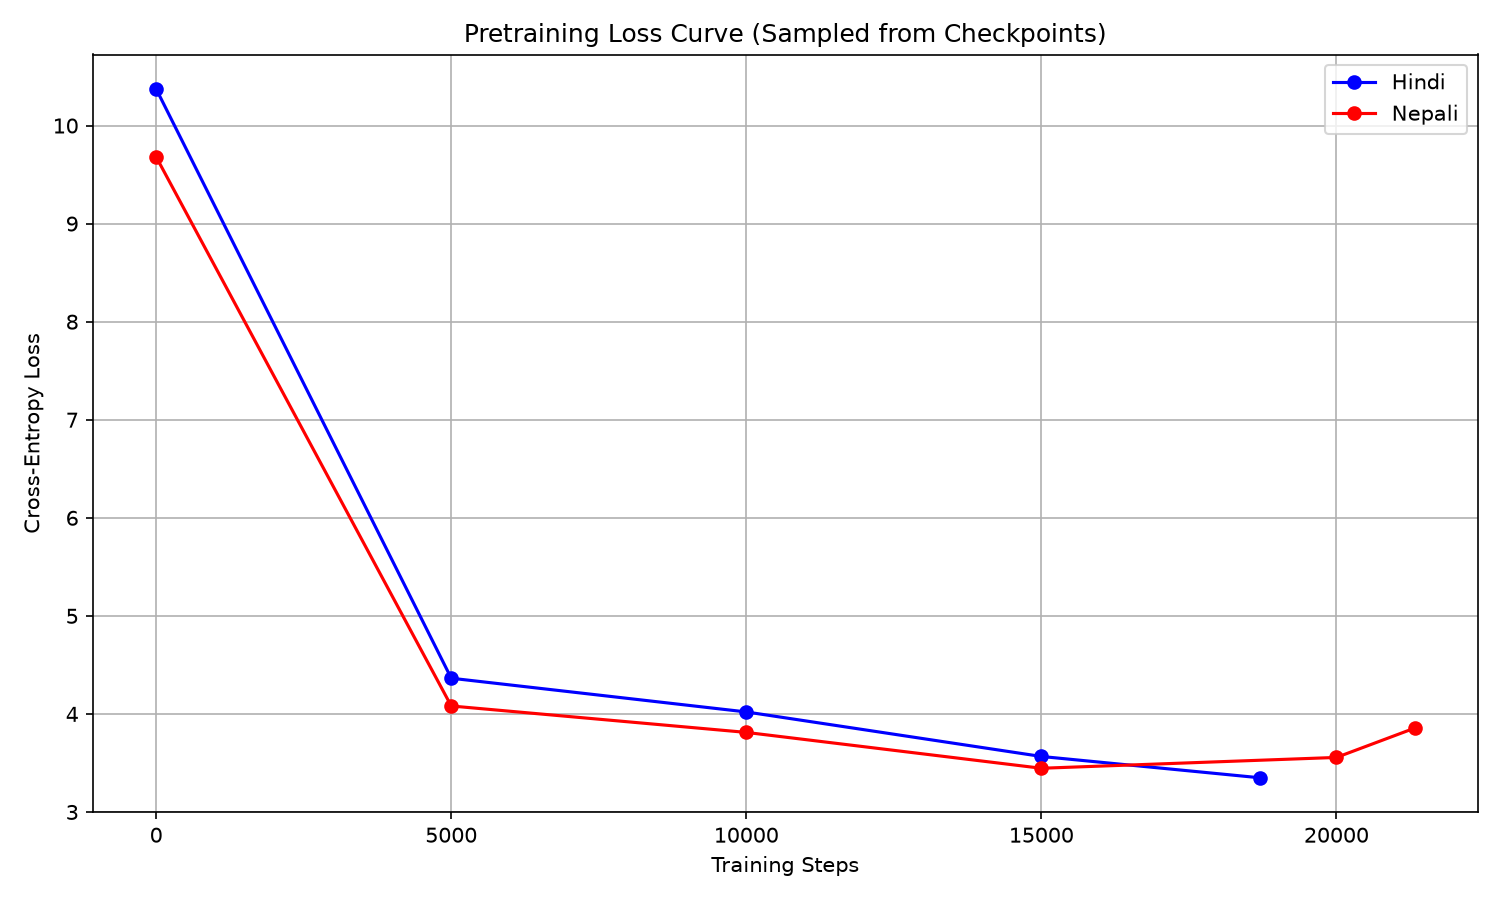
\includegraphics[width=\columnwidth]{images/loss_curve.png}
\caption{Phase 2 pretraining loss curves for Hindi and Nepali.}
\label{fig:phase2_loss}
\end{figure}

\subsection{Evaluation Across Intrinsic and Generation Metrics}
Models were evaluated on their respective held-out test sets across intrinsic loss, open-ended generation, and repetition diagnostics.

\begin{table}[t]
\centering
\footnotesize
\setlength{\tabcolsep}{3.5pt}
\caption{Phase 2 Comprehensive Test Evaluation}
\label{tab:phase2_results}
\begin{tabularx}{\columnwidth}{@{}>{\raggedright\arraybackslash}Xcc@{}}
\toprule
\textbf{Metric} & \textbf{Hindi (Model H)} & \textbf{Nepali (Model L)} \\
\midrule
Cross-Entropy Loss & 4.0162 & \textbf{3.6299} \\
Perplexity (PPL) & 55.4911 & \textbf{37.7073} \\
Bits-Per-Byte (BPB) & 5.7942 & \textbf{5.2368} \\
BLEU-4 & \textbf{3.51} & 0.00 \\
chrF & \textbf{9.19} & 4.43 \\
ROUGE-L & 0.0612 & \textbf{0.0680} \\
Distinct-1 (Unigrams) & 0.1321 & \textbf{0.2551} \\
Distinct-2 (Bigrams) & 0.2671 & \textbf{0.3956} \\
Repetition Rate & 0.6738 & \textbf{0.5644} \\
\bottomrule
\end{tabularx}
\end{table}

\subsection{Critical Analysis of the Language Modeling Gap}
A naive inspection would attribute Model H's higher perplexity (55.49 vs. 37.71) purely to its larger vocabulary size (32k vs. 16k). However, \textbf{Bits-Per-Byte (BPB)} explicitly normalizes for vocabulary size and tokenizer fertility:
\begin{equation}
\text{BPB} = \frac{\mathcal{L}_{\text{val}}}{\ln 2} \times \frac{N_{\text{tokens}}}{N_{\text{bytes}}}
\end{equation}
Even after this normalization, Hindi's BPB (5.7942) remains higher than Nepali's (5.2368), confirming that vocabulary dimensionality is an incomplete explanation.

The true driver is a pronounced \textbf{generalization and overfitting gap}: Hindi's training loss dropped to $\sim 3.35$ while its validation loss plateaued at $4.02$---a generalization gap of $\mathbf{0.67}$ (compared to a much tighter $\mathbf{0.32}$ gap in Nepali, from $3.31$ train to $3.63$ val). Because both models were trained without Dropout (relying solely on Weight Decay), Hindi's higher parameter capacity (36.84M vs. 28.65M) memorized local stylistic patterns on the finite training budget. Concurrently, generation metrics reveal that Model H maintained significantly stronger multi-token grammatical coherence (BLEU-4 of 3.51 vs. 0.00; chrF of 9.19 vs. 4.43), demonstrating that Nepali's lower cross-entropy was bolstered by predicting predictable inflectional morphemes without forming fluent long-range sentential syntax.

\subsection{Qualitative Generation Analysis Across Temperatures}
Continuations were generated from validation prompts across temperatures $T \in \{0.5, 1.0, 1.5\}$:
\begin{itemize}[noitemsep,leftmargin=*]
    \item \textbf{Low Temperature ($T=0.5$):} Both models exhibit high repetition loops (67.4\% Hindi, 56.4\% Nepali). Small 30M models quickly exhaust shallow local context and get trapped in cyclical postposition loops.
    \item \textbf{Balanced ($T=1.0$):} Hindi produces coherent domain sentences (\textit{"Bharat ek desh nahi ho paya hai aur ek rozgar wala desh hona hai..."}), maintaining correct SOV verbal agreements.
    \item \textbf{High Entropy ($T=1.5$):} Hallucinations emerge; Hindi emits phonetic transliterations of Latin technical terms, while Nepali exhibits random morphological agglutination.
\end{itemize}

\section{Phase 2 Multi-Head Attention Analysis}

In direct response to evaluation feedback, attention distributions were extracted across \textbf{all 6 layers and all 8 heads (48 heads per model, 96 attention heads total)} on benchmark sentences:
\begin{itemize}[noitemsep,leftmargin=*]
    \item \textbf{Hindi Benchmark:} \textit{"Bharat ek bahut hi sundar aur vishal desh hai."} (10 tokens)
    \item \textbf{Nepali Benchmark:} \textit{"Nepal ek dherai sundar ra vishal desh ho."} (9 tokens)
\end{itemize}

\subsection{Attention Coordinate System (X and Y Axes)}
In all attention heatmaps presented, the attention matrix $A \in \mathbb{R}^{T \times T}$ follows the standard Cartesian convention:
\begin{itemize}[noitemsep,leftmargin=*]
    \item \textbf{X-Axis (Horizontal / Columns $j$):} Represents the \textbf{Key Token ($K_j$)} / \textbf{Attended-to Context Token}. This is the historical token receiving attention, indexed from $j=0$ (left) to $j=T-1$ (right).
    \item \textbf{Y-Axis (Vertical / Rows $i$):} Represents the \textbf{Query Token ($Q_i$)} / \textbf{Attending Position / Currently Generating Token}, indexed from $i=0$ (top) to $i=T-1$ (bottom).
    \item \textbf{Cell $(i, j)$:} Softmax attention probability $A_{ij} \in [0, 1]$ indicating how much token $i$ attends to token $j$. Every horizontal row sums strictly to 1.0 ($\sum_{j=0}^{i} A_{ij} = 1.0$).
    \item \textbf{Upper Triangular Region ($j > i$):} Strictly zero (solid dark purple) due to the autoregressive causal mask enforcing that future tokens are invisible ($-\infty$ pre-softmax).
\end{itemize}

\subsection{Information-Theoretic Diagnostic Metrics}
For each head $h$ at layer $l$, two metrics were computed:
\begin{enumerate}[noitemsep,leftmargin=*]
    \item \textbf{Mean Shannon Entropy ($\bar{\mathcal{H}}$):}
    $\bar{\mathcal{H}} = -\frac{1}{T} \sum_{i=0}^{T-1} \sum_{j=0}^{i} A_{ij} \log_2 (A_{ij} + \epsilon)$. Low entropy indicates sharp focus (sinks or local syntax); high entropy indicates diffuse context pooling.
    \item \textbf{Mean Attention Distance ($\bar{D}$):}
    $\bar{D} = \frac{1}{T} \sum_{i=0}^{T-1} \sum_{j=0}^{i} A_{ij} \cdot (i - j)$. Measures the average backwards token span. $\bar{D} < 1.5$ is local; $\bar{D} > 3.0$ is global.
\end{enumerate}

\begin{table}[t]
\centering
\footnotesize
\setlength{\tabcolsep}{2.5pt}
\caption{Layer-Wise Aggregate Attention Trajectory (All 48 Heads)}
\label{tab:layer_trajectory}
\begin{tabularx}{\columnwidth}{@{}>{\raggedright\arraybackslash}Xcccc@{}}
\toprule
& \multicolumn{2}{c}{\textbf{Hindi (Model H)}} & \multicolumn{2}{c}{\textbf{Nepali (Model L)}} \\
\cmidrule(lr){2-3} \cmidrule(lr){4-5}
\textbf{Layer} & \textbf{Entropy} & \textbf{Distance} & \textbf{Entropy} & \textbf{Distance} \\
\midrule
Layer 0 & 0.7263 & 1.3076 & 0.7207 & 1.1908 \\
Layer 1 & 0.9303 & 1.9329 & 1.0150 & 1.9558 \\
Layer 2 & \textbf{1.2089}$^*$ & 2.4143 & \textbf{1.0065}$^*$ & 2.0341 \\
Layer 3 & 0.9430 & 2.7268 & 0.8203 & 2.6398 \\
Layer 4 & 0.8600 & 3.2971 & 0.7571 & 2.8805 \\
Layer 5 & \textbf{0.6923}$^\dagger$ & \textbf{3.4988}$^\ddagger$ & \textbf{0.5960}$^\dagger$ & \textbf{3.2427}$^\ddagger$ \\
\bottomrule
\multicolumn{5}{l}{\scriptsize $^*$Peak entropy; $^\dagger$minimum entropy; $^\ddagger$maximum distance.}
\end{tabularx}
\end{table}

\begin{table*}[t]
\centering
\scriptsize
\setlength{\tabcolsep}{2.0pt}
\caption{Complete 48-Head Quantitative Attention Diagnostics Across All Layers and Heads for Hindi and Nepali}
\label{tab:all_48_heads}
\begin{tabular}{ccccccc|ccccccc}
\toprule
\multicolumn{7}{c|}{\textbf{Early to Mid Layers (Layers 0, 1, 2)}} & \multicolumn{7}{c}{\textbf{Mid to Late Layers (Layers 3, 4, 5)}} \\
\textbf{L} & \textbf{H} & \textbf{Hi }$\mathcal{H}$ & \textbf{Hi }$\bar{D}$ & \textbf{Hi Role} & \textbf{Ne }$\mathcal{H}$ & \textbf{Ne }$\bar{D}$ & \textbf{L} & \textbf{H} & \textbf{Hi }$\mathcal{H}$ & \textbf{Hi }$\bar{D}$ & \textbf{Hi Role} & \textbf{Ne }$\mathcal{H}$ & \textbf{Ne }$\bar{D}$ \\
\midrule
L0 & H0 & 0.73 & 1.03 & Local n-gram & 1.07 & 1.44 & L3 & H0 & 1.01 & 3.11 & Global & 0.66 & 3.12 \\
L0 & H1 & 0.35 & 0.31 & Hyper-local & 0.47 & 0.61 & L3 & H1 & 0.84 & 1.78 & Phrase syntax & 1.04 & 2.50 \\
L0 & H2 & 0.28 & 0.47 & Hyper-local & 1.09 & 2.34 & L3 & H2 & 0.78 & 2.25 & Relational & 0.75 & 2.78 \\
L0 & H3 & 0.54 & 1.20 & Phrase syntax & 1.11 & 1.70 & L3 & H3 & 1.01 & 2.65 & Relational & 0.68 & 1.38 \\
L0 & H4 & 1.16 & 2.50 & Relational & 0.92 & 1.27 & L3 & H4 & 1.06 & 3.04 & Global & 0.79 & 3.19 \\
L0 & H5 & 1.02 & 1.88 & Phrase syntax & 0.54 & 1.21 & L3 & H5 & 0.92 & 2.73 & Relational & 0.96 & 2.84 \\
L0 & H6 & 1.14 & 1.91 & Diffuse syntax & 0.45 & 0.84 & L3 & H6 & 0.76 & 3.64 & Semantic & 0.79 & 3.08 \\
L0 & H7 & 0.59 & 1.16 & Local n-gram & 0.12 & 0.13 & L3 & H7 & 1.17 & 2.61 & Relational & 0.89 & 2.24 \\
\midrule
L1 & H0 & 0.95 & 2.23 & Relational & 1.09 & 2.36 & L4 & H0 & 1.09 & 3.23 & Global & 0.84 & 2.73 \\
L1 & H1 & 1.02 & 1.82 & Phrase syntax & 1.21 & 1.67 & L4 & H1 & 0.39 & 4.11 & Strong Sink & 0.83 & 3.10 \\
L1 & H2 & 0.78 & 1.37 & Phrase syntax & 0.93 & 2.09 & L4 & H2 & 0.89 & 3.03 & Semantic & 0.21 & 3.68 \\
L1 & H3 & 1.16 & 2.78 & Relational & 1.09 & 1.96 & L4 & H3 & 0.99 & 2.84 & Relational & 0.79 & 2.90 \\
L1 & H4 & 1.25 & 2.12 & Diffuse syntax & 1.09 & 2.51 & L4 & H4 & 1.20 & 2.85 & Relational & 0.71 & 3.16 \\
L1 & H5 & 0.88 & 2.11 & Phrase syntax & 1.24 & 2.35 & L4 & H5 & 0.73 & 3.03 & Semantic & 0.88 & 2.20 \\
L1 & H6 & 0.81 & 1.99 & Phrase syntax & 0.32 & 0.93 & L4 & H6 & 0.49 & 4.07 & Strong Sink & 1.03 & 2.51 \\
L1 & H7 & 0.59 & 1.06 & Local n-gram & 1.16 & 1.79 & L4 & H7 & 1.11 & 3.21 & Global & 0.76 & 2.77 \\
\midrule
L2 & H0 & 1.15 & 1.90 & Diffuse syntax & 1.16 & 2.14 & L5 & H0 & 0.74 & 3.73 & Semantic & 0.75 & 3.13 \\
L2 & H1 & 1.27 & 2.54 & Diffuse pool & 1.10 & 2.64 & L5 & H1 & 1.11 & 2.08 & Diffuse syntax & 0.44 & 3.57 \\
L2 & H2 & 1.16 & 3.02 & Global & 0.58 & 0.96 & L5 & H2 & 1.03 & 3.13 & Global & 0.16 & 3.88 \\
L2 & H3 & 1.24 & 2.10 & Diffuse syntax & 0.85 & 1.36 & L5 & H3 & 0.97 & 2.95 & Relational & 0.68 & 3.29 \\
L2 & H4 & 1.34 & 2.33 & Diffuse pool & 1.20 & 2.09 & L5 & H4 & 0.52 & 4.08 & Strong Sink & 1.00 & 2.38 \\
L2 & H5 & 1.33 & 2.96 & Diffuse pool & 1.26 & 2.33 & L5 & H5 & 0.16 & 4.33 & Extreme Sink & 0.40 & 3.66 \\
L2 & H6 & 1.31 & 2.28 & Diffuse pool & 1.07 & 2.18 & L5 & H6 & 0.17 & 4.30 & Extreme Sink & 0.43 & 3.46 \\
L2 & H7 & 0.88 & 2.18 & Phrase syntax & 0.83 & 2.56 & L5 & H7 & 0.84 & 3.39 & Semantic & 0.91 & 2.57 \\
\bottomrule
\end{tabular}
\end{table*}

\begin{figure*}[t]
\centering
\begin{subfigure}[b]{0.49\textwidth}
    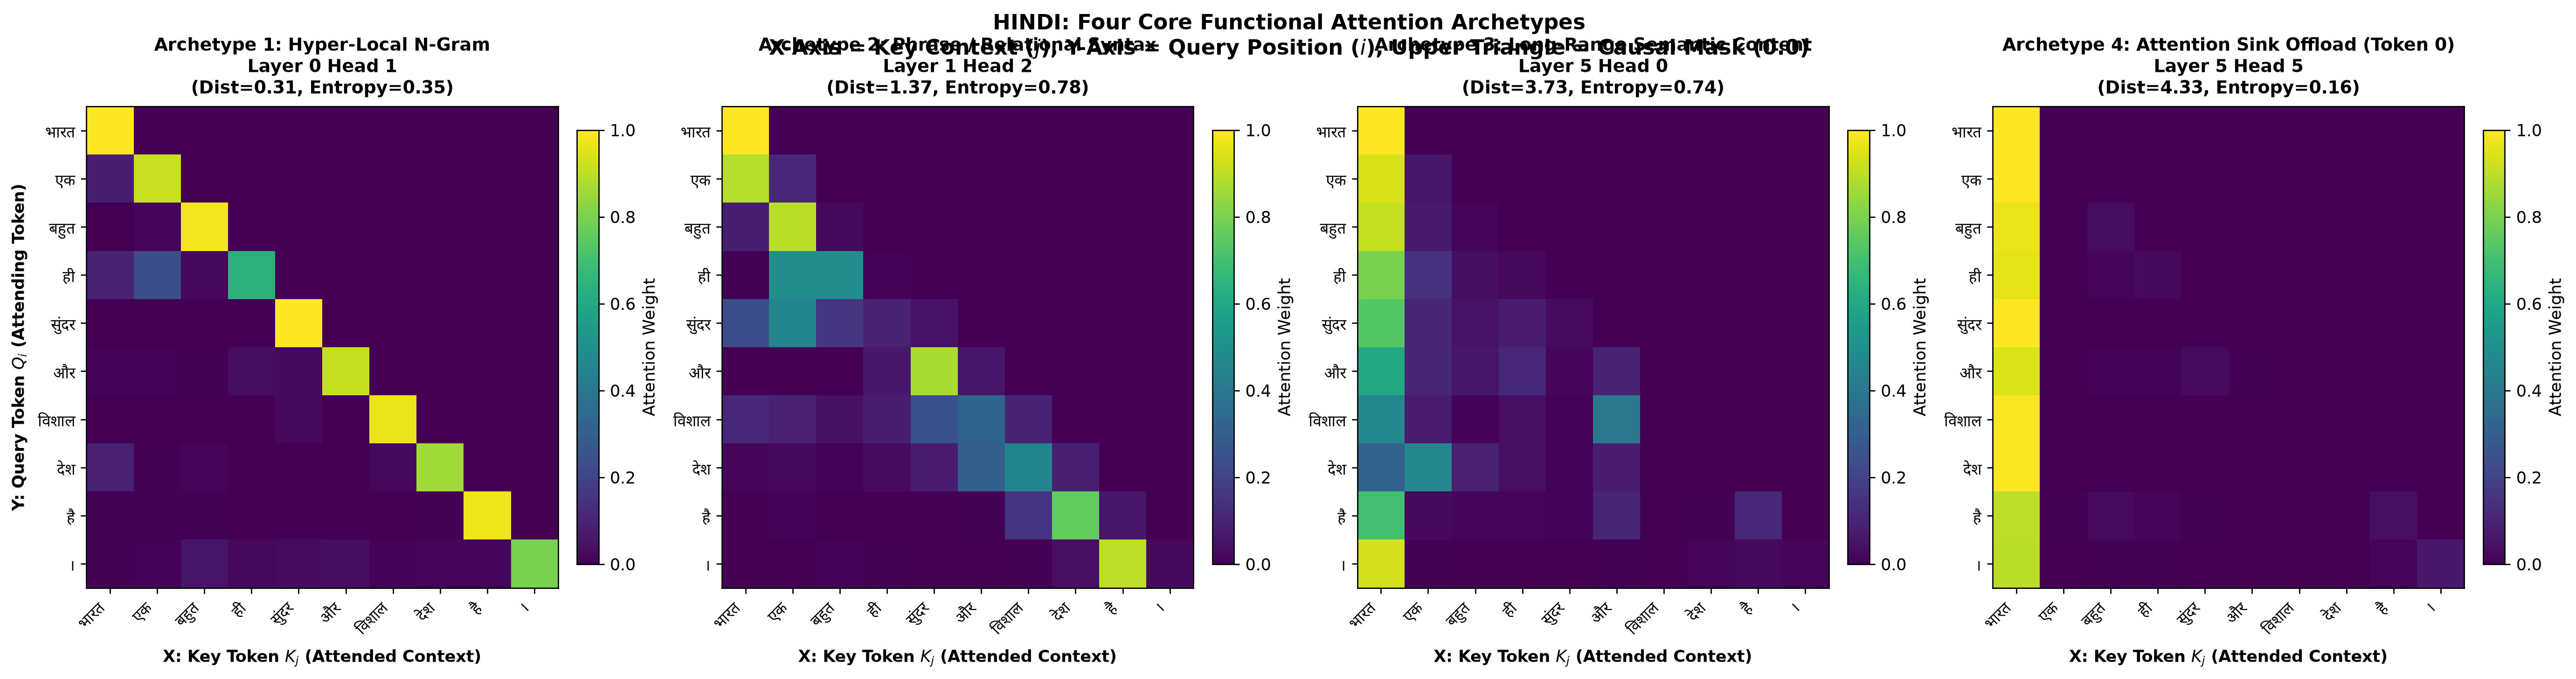
\includegraphics[width=\textwidth]{images/separate_heads_hindi_archetypes.png}
    \caption{Hindi: Four Core Functional Attention Archetypes}
\end{subfigure}
\hfill
\begin{subfigure}[b]{0.49\textwidth}
    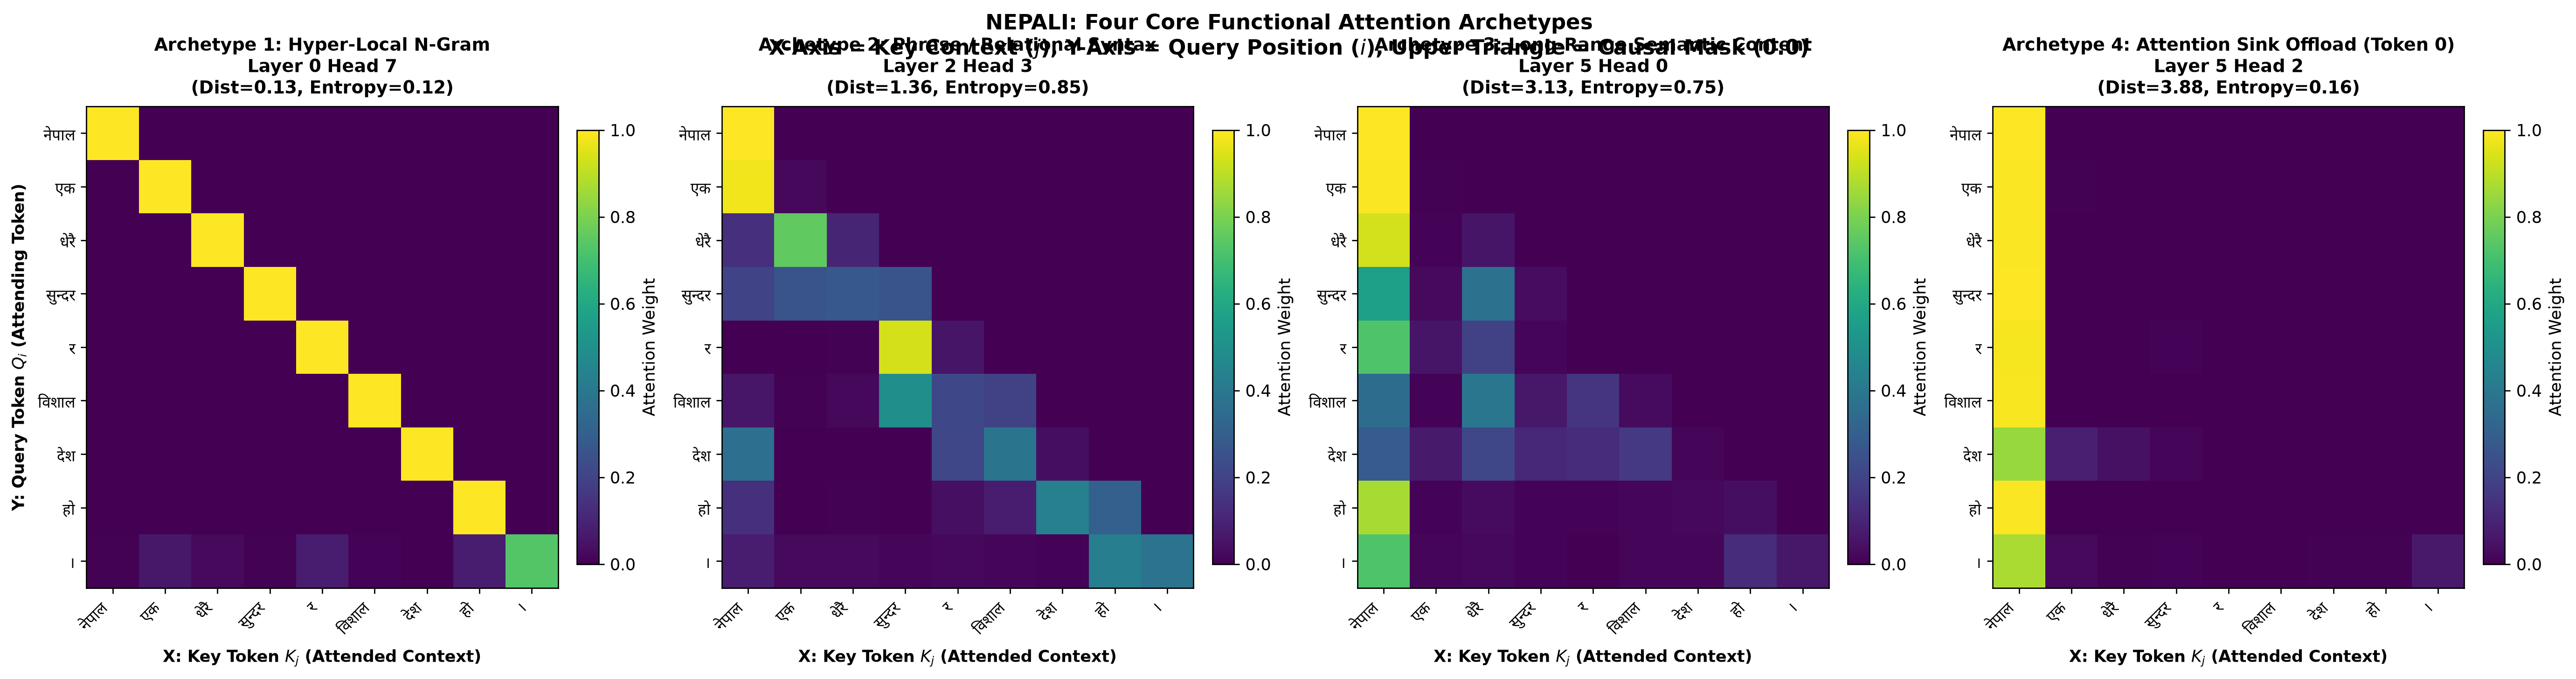
\includegraphics[width=\textwidth]{images/separate_heads_nepali_archetypes.png}
    \caption{Nepali: Four Core Functional Attention Archetypes}
\end{subfigure}
\caption{Separate high-resolution attention heatmaps illustrating the four primary functional archetypes discovered in our models. $X$-axis = Key token $K_j$ (context receiving attention); $Y$-axis = Query token $Q_i$ (attending position). Dark purple upper triangle = causal mask ($0.0$).}
\label{fig:archetype_heatmaps}
\end{figure*}

\subsection{Four Core Functional Attention Archetypes}
Figure~\ref{fig:archetype_heatmaps} displays separate high-resolution heatmaps for the four primary archetypes identified across both models:
\begin{enumerate}[noitemsep,leftmargin=*]
    \item \textbf{Hyper-Local N-Gram Heads (e.g., Hindi L0H1, Nepali L0H7):} Sharp diagonal concentration ($j=i, i-1$) with distances $\le 0.31$ and low entropy ($\le 0.35$). These heads extract adjacent subword n-grams.
    \item \textbf{Phrase-Level Relational Syntax (e.g., Hindi L1H2, Nepali L2H3):} Look back 1--2 tokens (distance $\sim 1.37$) to bind modifiers and adjectives (\textit{"sundar"} + \textit{"ra"} + \textit{"vishal"} $\rightarrow$ \textit{"desh"}).
    \item \textbf{Long-Range Semantic Content (e.g., Hindi L5H0, Nepali L5H0):} Span the full sentence (distance $\sim 3.73$, entropy $\sim 0.74$), routing information from subjects and predicative adjectives to sentence-final verbs.
    \item \textbf{Attention Sinks (e.g., Hindi L5H5, Nepali L5H2):} Intense vertical stripes down column 0 (\textit{"Bharat"} / \textit{"Nepal"}) with extreme distances ($>3.88$) and ultra-low entropy ($\sim 0.16$). Because Softmax enforces $\sum_j A_{ij} = 1.0$, queries that find no relevant syntactic dependency dump surplus attention mass into token 0 as a harmless "no-op" valve.
\end{enumerate}

\subsection{Master 6x8 Attention Grids}
Figure~\ref{fig:master_grids} presents the complete 48-head attention maps for Hindi and Nepali, displaying all 6 layers (rows) and 8 heads (columns) simultaneously. In both languages, the transition from local diagonal banding (top rows) to vertical attention sink columns (bottom rows) is universally evident.

\begin{figure*}[t]
\centering
\begin{subfigure}[b]{0.49\textwidth}
    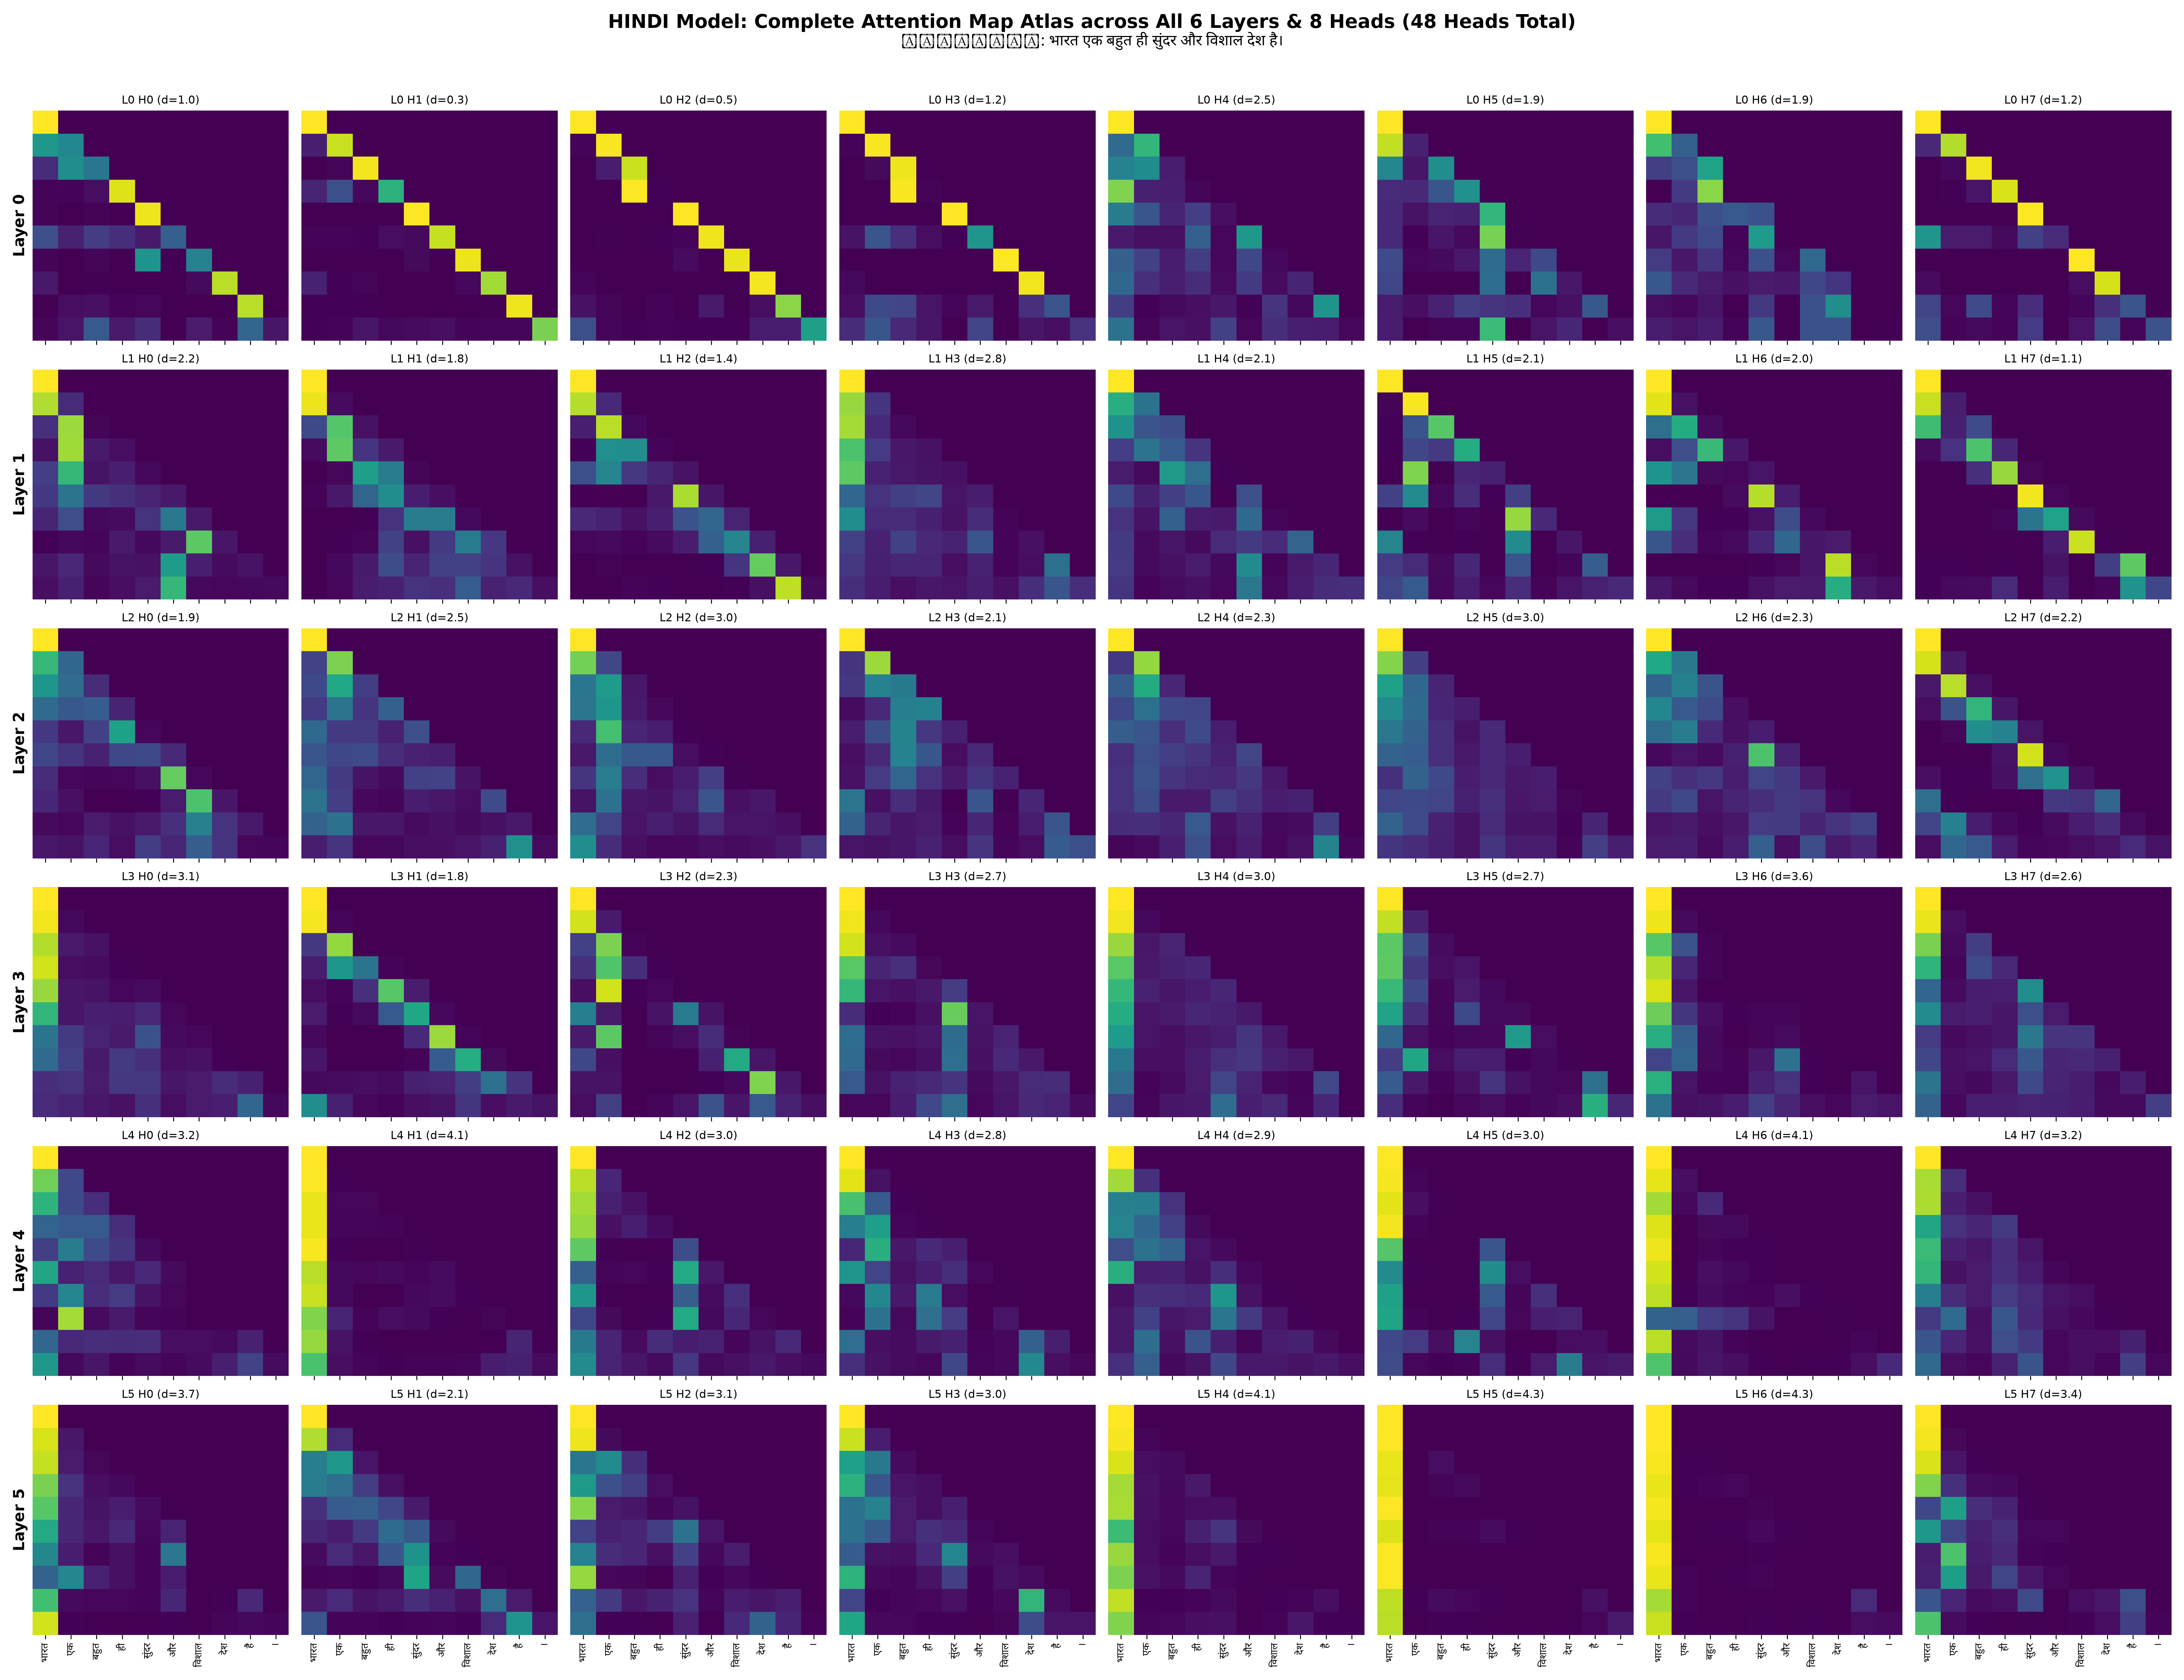
\includegraphics[width=\textwidth]{images/all_layers_all_heads_hindi.png}
    \caption{Hindi: All 48 Attention Heads (6 Layers $\times$ 8 Heads)}
\end{subfigure}
\hfill
\begin{subfigure}[b]{0.49\textwidth}
    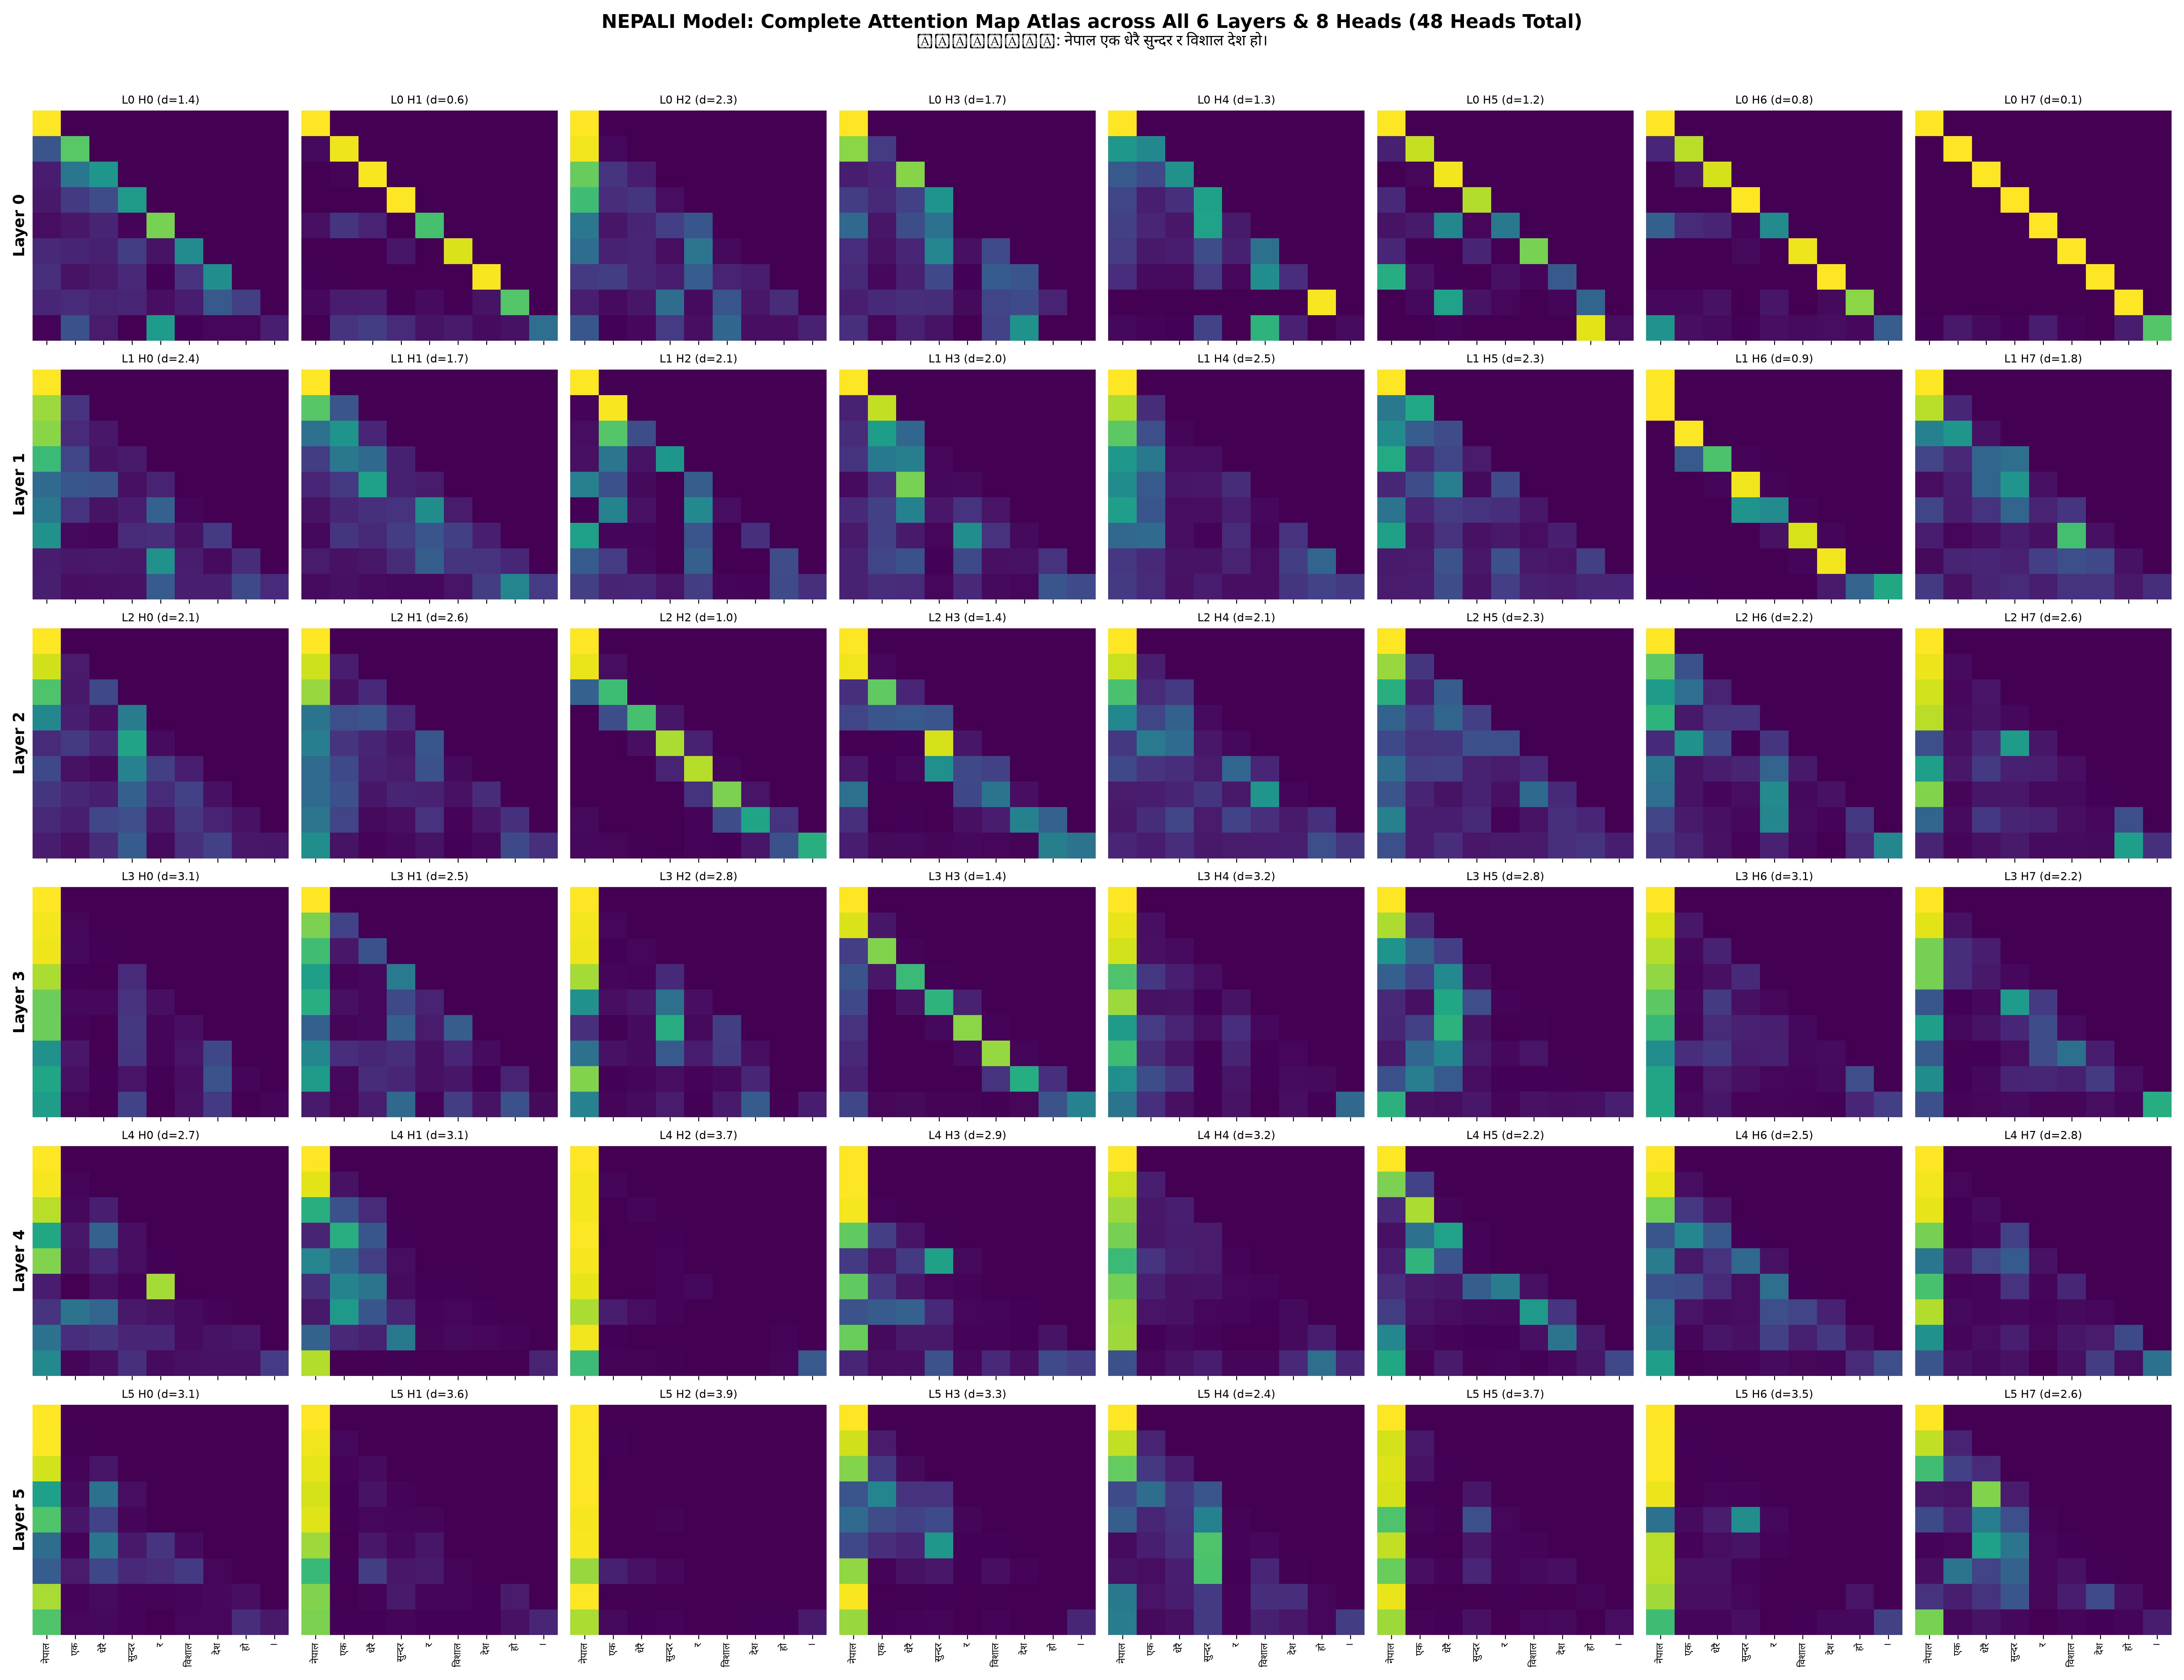
\includegraphics[width=\textwidth]{images/all_layers_all_heads_nepali.png}
    \caption{Nepali: All 48 Attention Heads (6 Layers $\times$ 8 Heads)}
\end{subfigure}
\caption{Complete 48-head attention heatmaps across all 6 layers and 8 heads for Hindi and Nepali. Rows correspond to Layers 0--5; columns correspond to Heads 0--7. Both models demonstrate uniform structural evolution: early diagonal localization transitioning to late-layer semantic routing and first-token attention sinks.}
\label{fig:master_grids}
\end{figure*}

\section{Phase 3: Reasoning Finetuning and Attention Redistribution}

\subsection{Synthetic Reasoning Dataset Construction}
To evaluate compositional and multi-step reasoning without contamination from public English benchmarks, custom synthetic reasoning datasets were generated in native Hindi and Nepali phrasing.

\subsubsection{Task Formulation}
\begin{itemize}[noitemsep,leftmargin=*]
    \item \textbf{Direct Comparison (2 Entities):} Two entities are assigned numeric attributes (height, age, quantity), and the model must identify the extreme entity.
    \item \textbf{Transitive Chaining (3 Entities):} Multi-hop relational chaining without explicit numbers ($A > B$ and $B > C$; who is greatest/least?).
\end{itemize}

\subsubsection{Strict Leakage Controls}
To guarantee zero-shot generalization without memorization:
\begin{itemize}[noitemsep,leftmargin=*]
    \item \textbf{Disjoint Entity Partition:} 10 out of 50 entity names (20\%) were strictly held out for testing only.
    \item \textbf{100\% Held-Out Test Attribute:} The attributes \textit{height}, \textit{age}, and \textit{quantity} were used exclusively in training/validation. 100\% of the 400 test examples evaluated the held-out attribute \textbf{\textit{price}} on the 10 held-out entity names.
    \item \textbf{Template Diversity:} Three distinct natural grammatical templates per task per language.
\end{itemize}

\begin{table}[t]
\centering
\footnotesize
\setlength{\tabcolsep}{2.0pt}
\caption{Phase 3 Reasoning Dataset Partitions}
\label{tab:reasoning_splits}
\begin{tabularx}{\columnwidth}{@{}>{\raggedright\arraybackslash}lrrr>{\raggedright\arraybackslash}X@{}}
\toprule
\textbf{Split} & \textbf{Dir.} & \textbf{Trans.} & \textbf{Total} & \textbf{Domain \& Entities} \\
\midrule
Train & 1,800 & 1,800 & 3,600 & Height, Age, Qty (40 Seen) \\
Val & 200 & 200 & 400 & Height, Age, Qty (40 Seen) \\
\textbf{Test} & 200 & 200 & \textbf{400} & \textbf{Price Only (10 Held-out)} \\
\bottomrule
\end{tabularx}
\end{table}

\subsection{Supervised Finetuning Protocol}
Finetuning started from each model's Phase 2 pretrained checkpoint (\texttt{final.pt}).
\begin{itemize}[noitemsep,leftmargin=*]
    \item \textbf{Prompt Masking:} Cross-entropy loss was calculated exclusively on the answer entity tokens and the EOS token (\texttt{ignore\_index=-100} on prompt tokens).
    \item \textbf{Hyperparameters:} AdamW ($\text{lr}=2\times 10^{-5}, \beta_1=0.9, \beta_2=0.95, \text{wd}=0.01$), batch size 4, gradient accumulation 16 (effective batch 64), 5 epochs, cosine schedule, gradient clipping at 1.0.
\end{itemize}

\begin{figure}[t]
\centering
\begin{subfigure}[b]{0.48\columnwidth}
    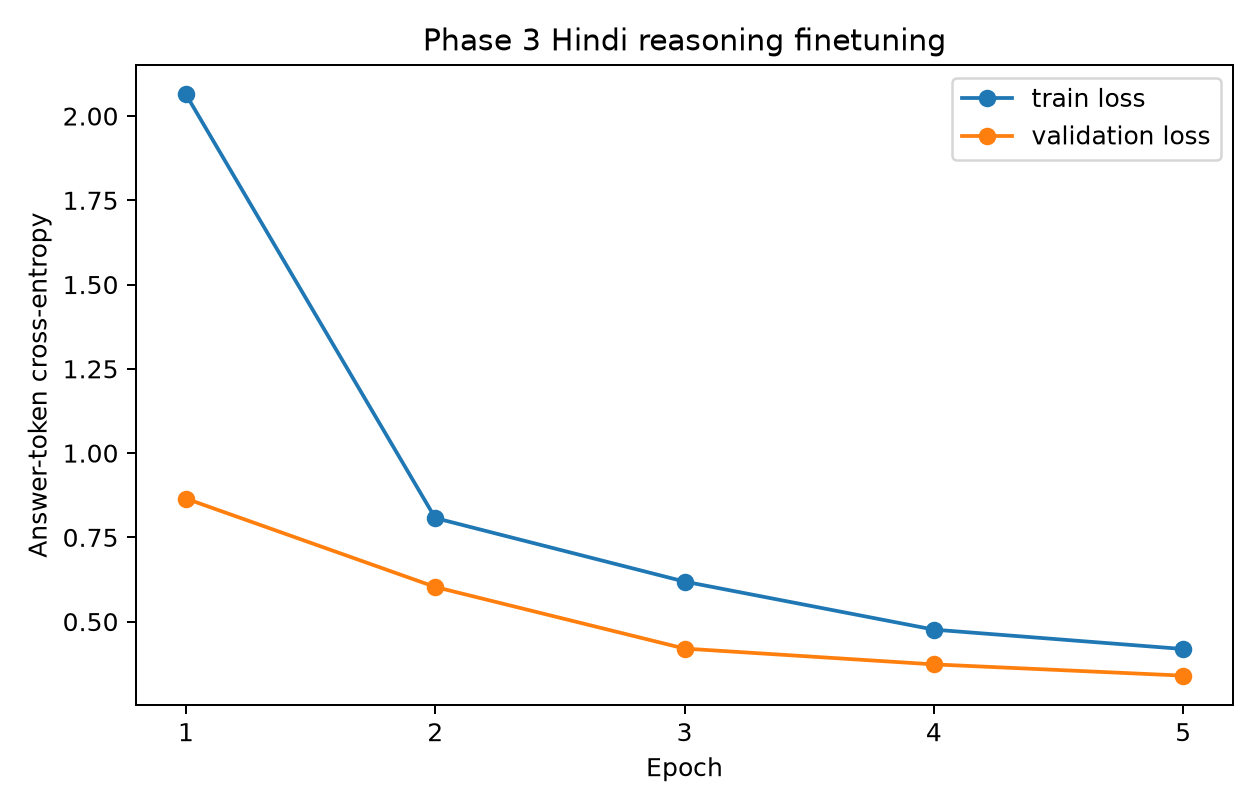
\includegraphics[width=\textwidth]{images/phase3_hindi_finetuning_loss.png}
    \caption{Hindi SFT Loss}
\end{subfigure}
\hfill
\begin{subfigure}[b]{0.48\columnwidth}
    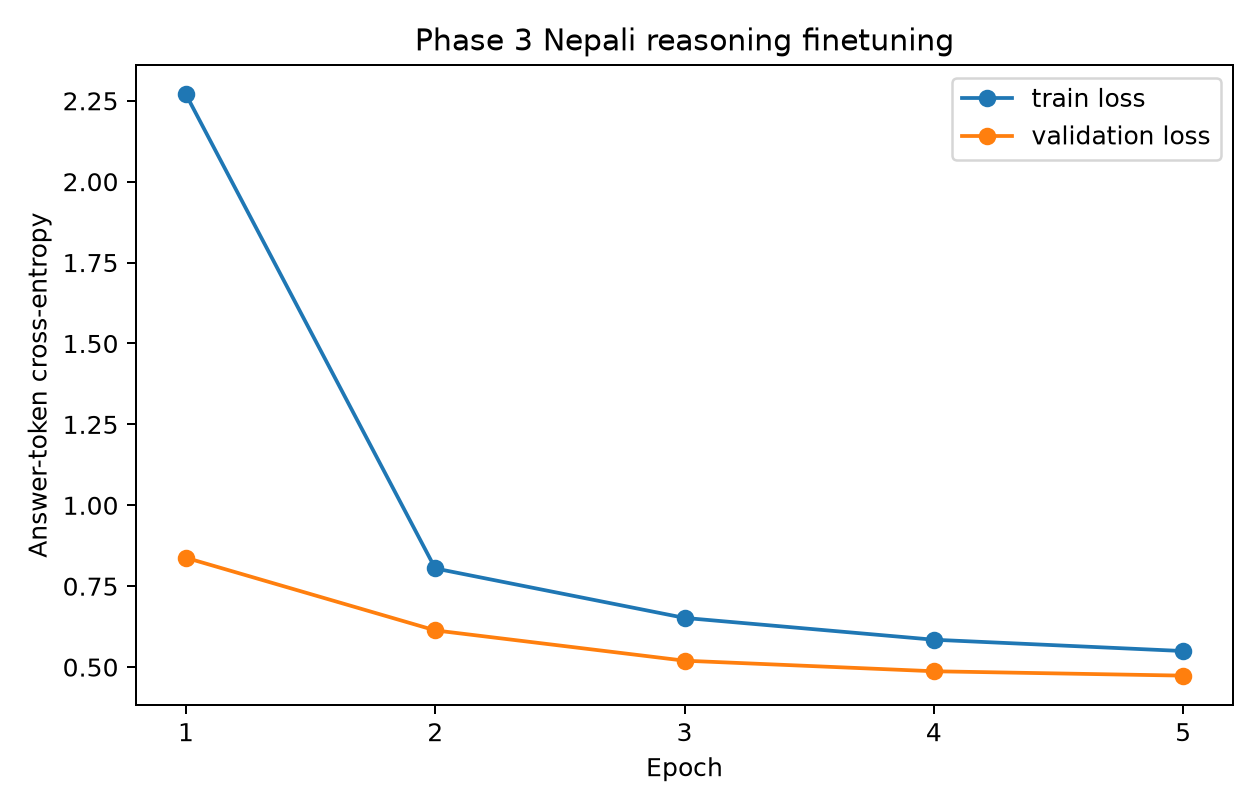
\includegraphics[width=\textwidth]{images/phase3_nepali_finetuning_loss.png}
    \caption{Nepali SFT Loss}
\end{subfigure}
\caption{Phase 3 supervised reasoning finetuning loss curves.}
\label{fig:phase3_finetune_loss}
\end{figure}

\subsection{Reasoning Evaluation Results}
Evaluation measured exact-match accuracy against held-out entities under greedy decoding.

\begin{table}[t]
\centering
\footnotesize
\setlength{\tabcolsep}{2.5pt}
\caption{Exact-Match Reasoning Accuracy: Pretrained vs. Finetuned}
\label{tab:reasoning_results}
\begin{tabularx}{\columnwidth}{@{}>{\raggedright\arraybackslash}Xcccc@{}}
\toprule
& \multicolumn{2}{c}{\textbf{Hindi}} & \multicolumn{2}{c}{\textbf{Nepali}} \\
\cmidrule(lr){2-3} \cmidrule(lr){4-5}
\textbf{Task Category} & \textbf{Pre} & \textbf{SFT} & \textbf{Pre} & \textbf{SFT} \\
\midrule
Direct Comp. (200) & 21.0\% & \textbf{52.0\%} & 1.0\% & \textbf{28.5\%} \\
Transitive Chain (200) & 3.0\% & \textbf{43.5\%} & 0.0\% & \textbf{20.5\%} \\
\midrule
\textbf{Overall Acc. (400)} & \textbf{12.0\%} & \textbf{47.75\%} & \textbf{0.5\%} & \textbf{24.50\%} \\
\textbf{Absolute Gain} & \multicolumn{2}{c}{\textbf{+35.75\%}} & \multicolumn{2}{c}{\textbf{+24.00\%}} \\
\bottomrule
\end{tabularx}
\end{table}

\subsection{Qualitative Error Analysis and Failure Modes}
\begin{itemize}[noitemsep,leftmargin=*]
    \item \textbf{Resolved Reasoning:} In Hindi transitive chains ($A > B$ and $B > C$), the pretrained model emitted repetitive subwords. The SFT model correctly resolved the two-hop relation to output entity $A$.
    \item \textbf{Persistent Failure Mode (One-Hop Hopping):} In transitive queries asking for the minimum entity in $A > B > C$, errors predominantly output intermediate entity $B$ rather than $C$. The model recognized the comparative context but performed a local one-hop transition instead of completing the full chain.
\end{itemize}

\subsection{Post-Finetuning Attention Redistribution}
Analyzing attention heatmaps before and after SFT on reasoning prompts revealed significant structural adaptations:
\begin{itemize}[noitemsep,leftmargin=*]
    \item \textbf{Nepali Relational Head (L5H0):} Contracted its receptive distance from \textbf{10.25 to 6.55 tokens}, while entropy expanded from \textbf{1.23 to 1.69}, sharpening its focus directly onto relational entity pairs.
    \item \textbf{Dismantling Pathological Sinks (Nepali L5H2):} In pretrained Model L, Layer 5 Head 2 acted as an extreme sink (entropy 0.68, distance 12.48 tokens), dumping mass onto delimiters. Finetuning broke this pathological sink: distance contracted to \textbf{8.20 tokens} and entropy rose to \textbf{0.87}, redirecting capacity to semantic tokens.
\end{itemize}

\begin{figure}[t]
\centering
\begin{subfigure}[b]{0.48\columnwidth}
    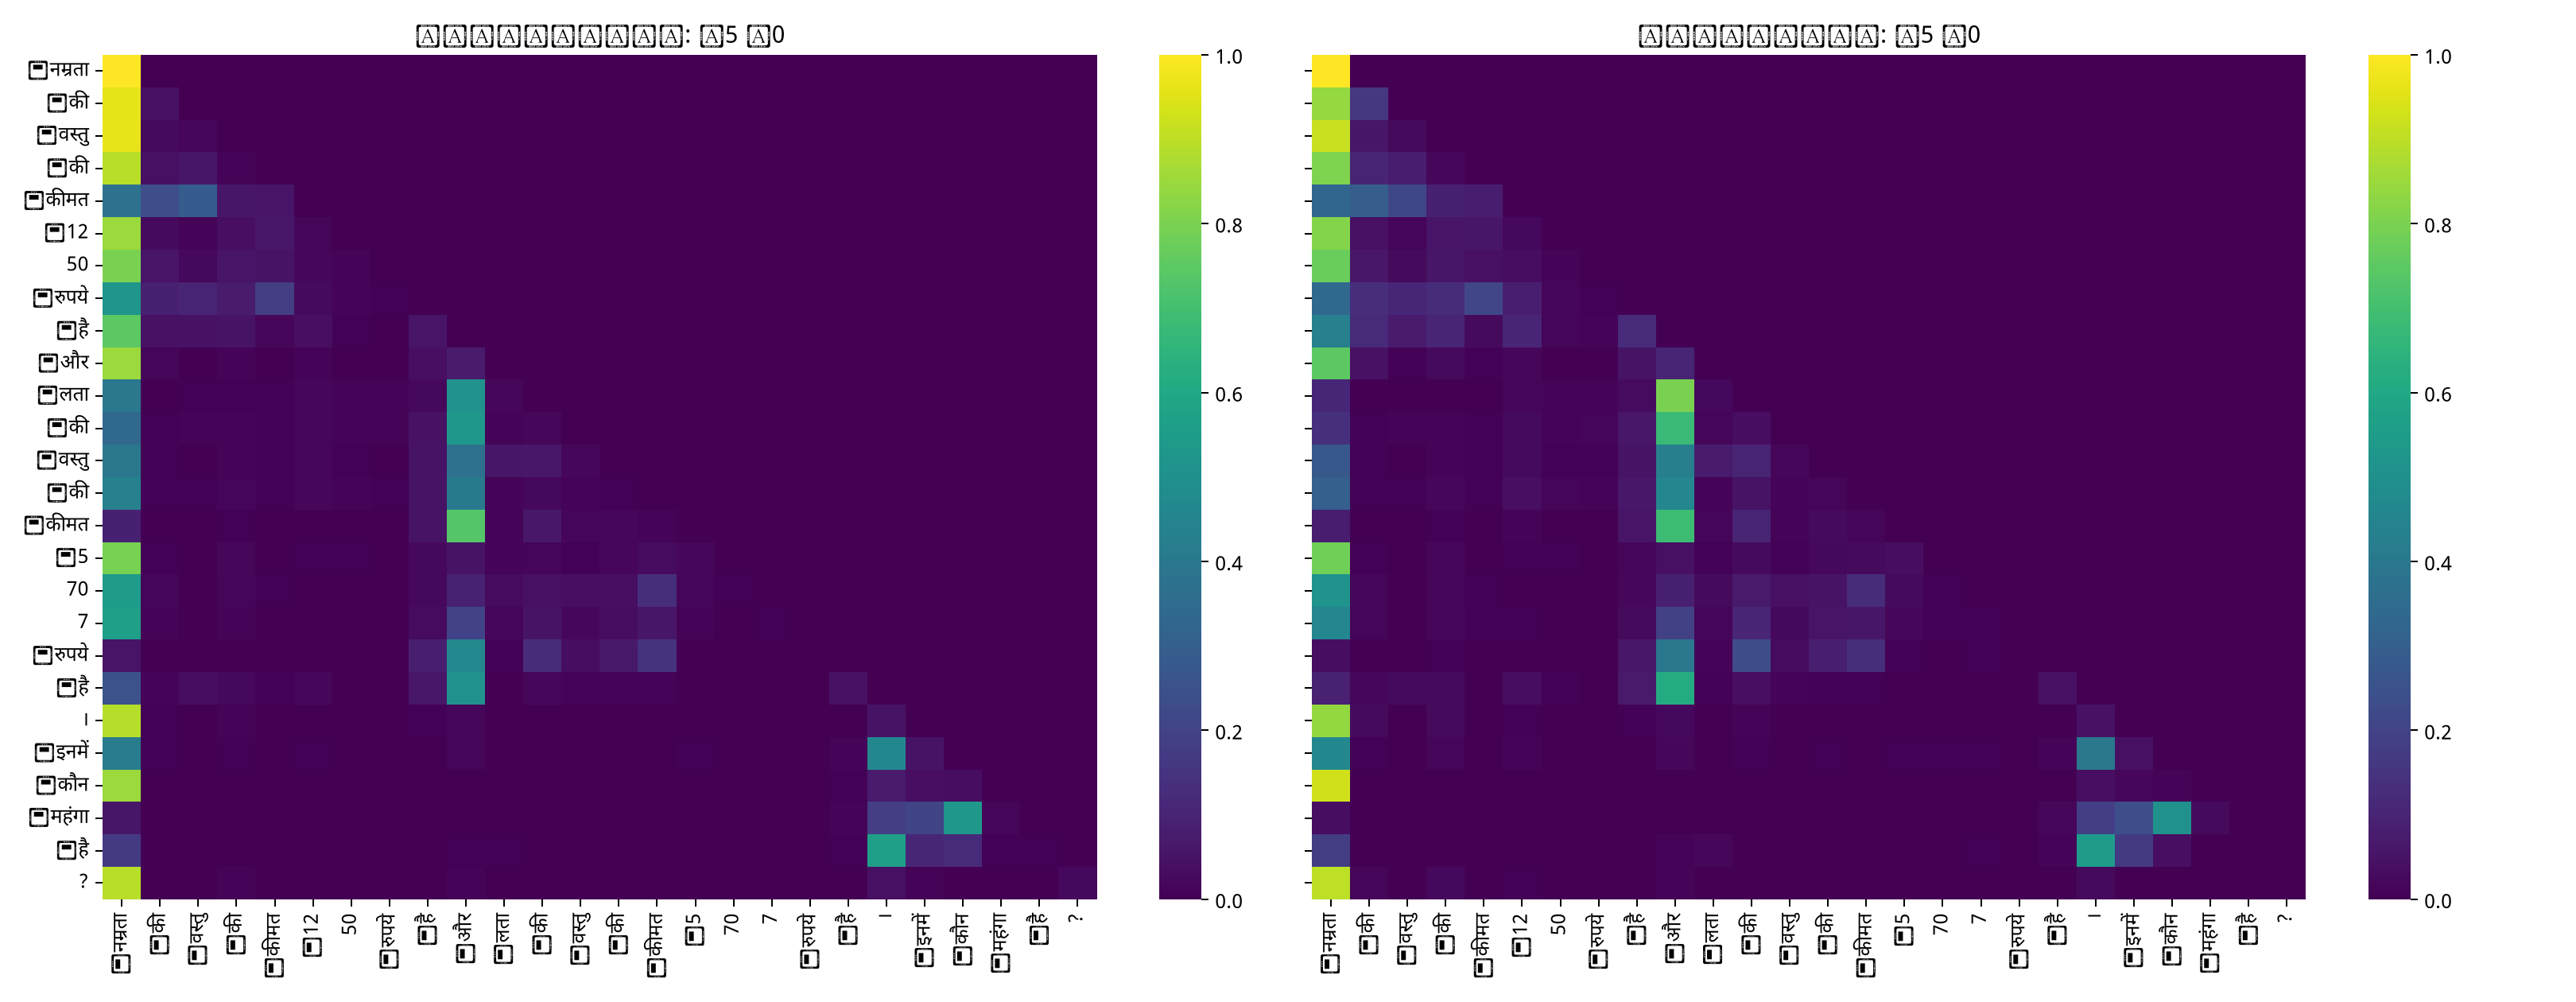
\includegraphics[width=\textwidth]{images/phase3/hindi/L5_H0_pretrained_vs_finetuned.png}
    \caption{Hindi: Pre vs. SFT (L5 H0)}
\end{subfigure}
\hfill
\begin{subfigure}[b]{0.48\columnwidth}
    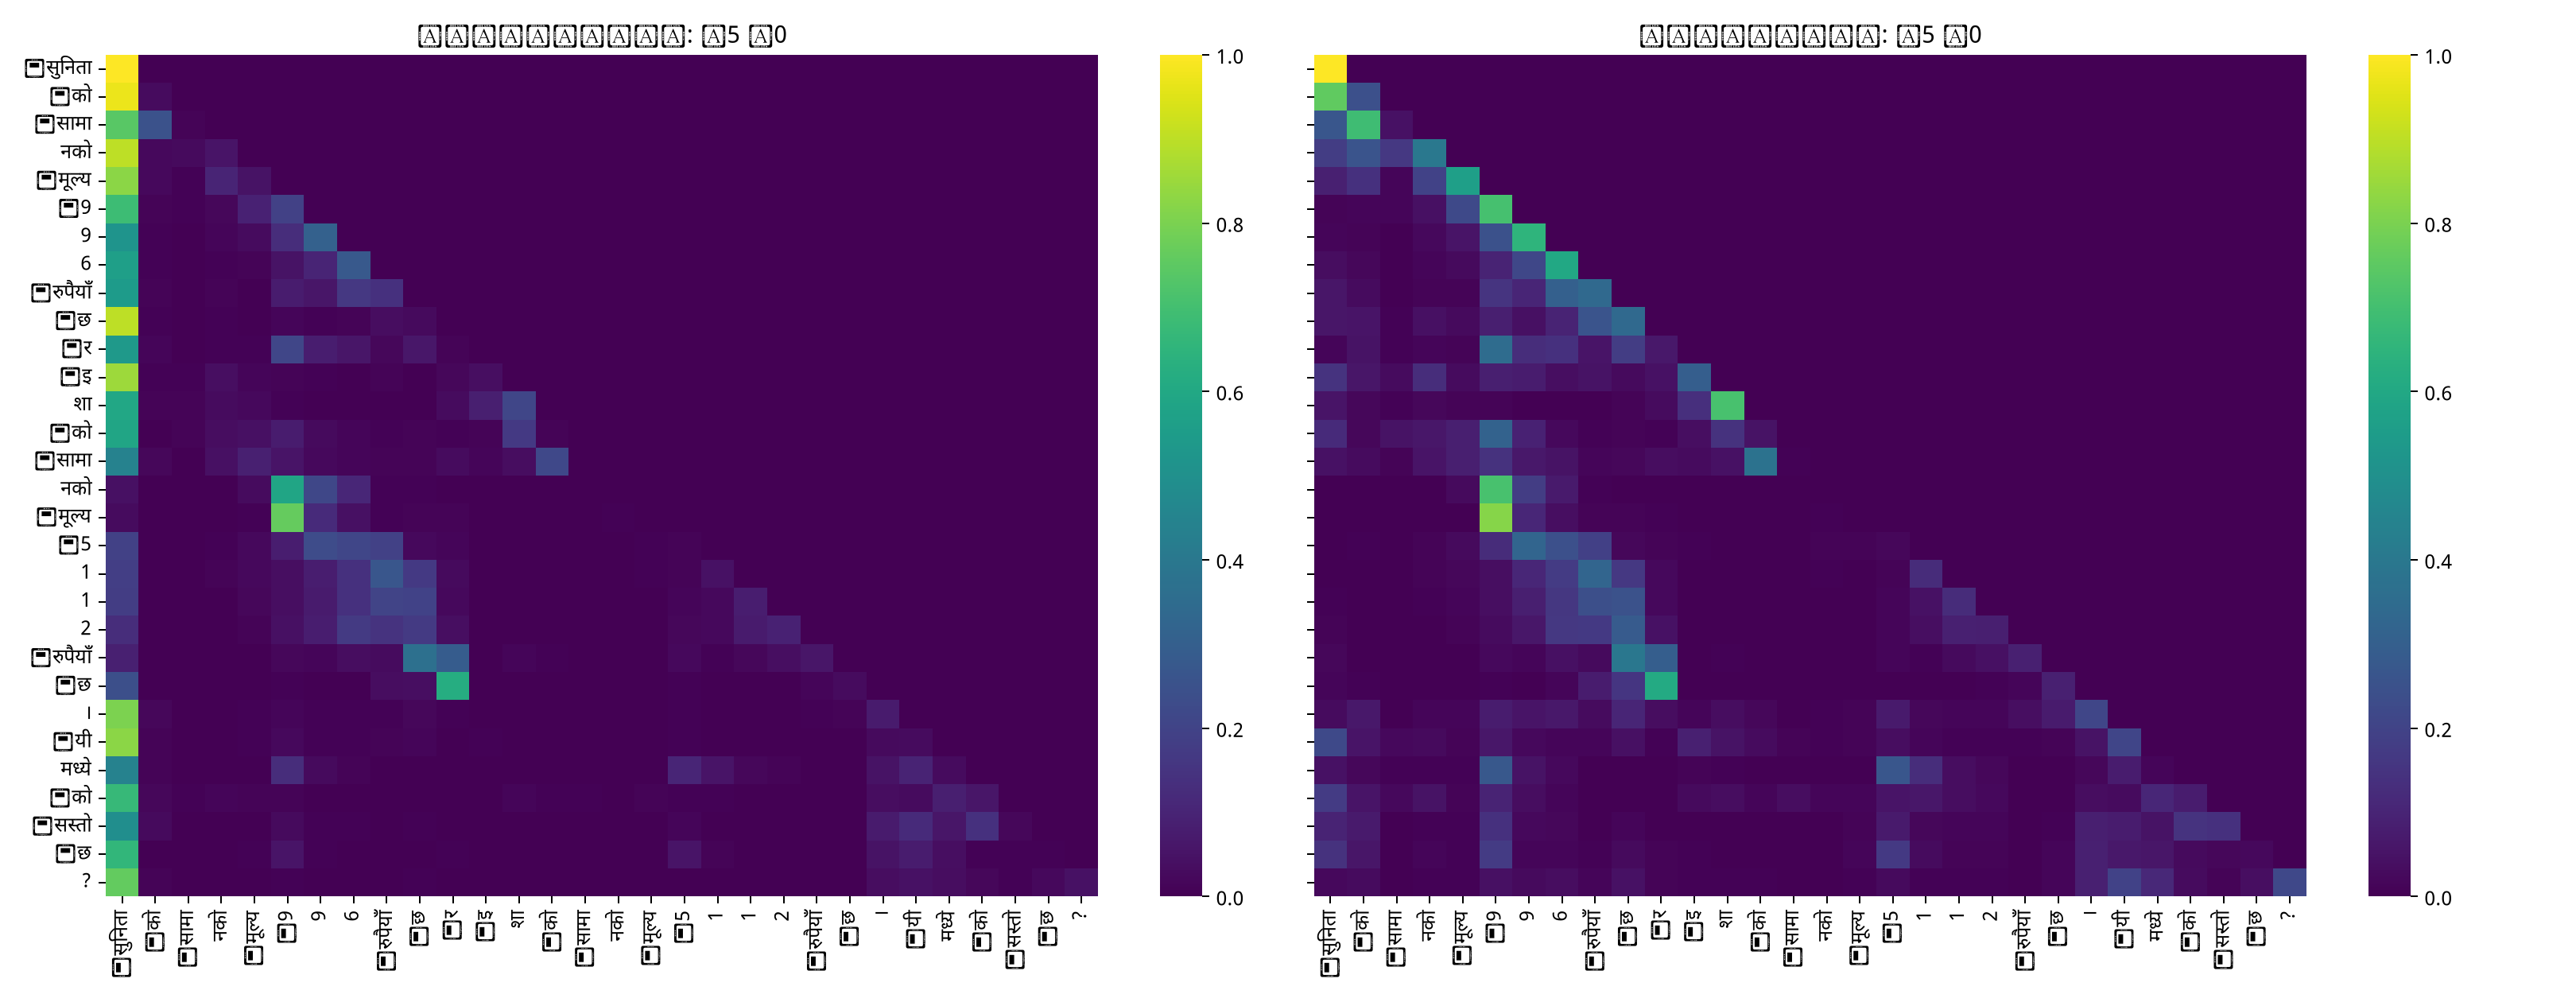
\includegraphics[width=\textwidth]{images/phase3/nepali/L5_H0_pretrained_vs_finetuned.png}
    \caption{Nepali: Pre vs. SFT (L5 H0)}
\end{subfigure}
\caption{Pretrained vs. Finetuned attention maps on reasoning prompts.}
\label{fig:phase3_attn_comparison}
\end{figure}

\section{Bonus: Positional Ablation Study (No Positional Embeddings)}

\subsection{Theoretical Rationale: Order Invariance}
Without positional embeddings, self-attention computes:
\begin{equation}
\text{Attn}(X) = \text{softmax}\left( \frac{(XW_Q)(XW_K)^T}{\sqrt{d_k}} + M \right) (XW_V)
\end{equation}
The dot product between token $t$ and token $s$ is $x_t W_Q W_K^T x_s^T$, which is **completely invariant to the sequence distance $|t - s|$**. Aside from the triangular causal mask $M$, all previous tokens in the sequence are treated as an unordered multiset.

\subsection{Empirical Invariance Proof and Evaluation}
We implemented \texttt{LanguageModelNoPos}, retaining all 36.84M parameters, 6 layers, 8 heads, 512 dimensions, RMSNorm, and SwiGLU FFN, but completely excising RoPE. In standard Model H, shifting relative token distance from 1 to 4 altered query-key dot products by \textbf{0.3394}. In the ablated model, the divergence was \textbf{0.0000}, confirming exact distance invariance.

The ablated model was trained on the Hindi corpus under identical hyperparameters and evaluated against standard Model H.

\begin{table}[t]
\centering
\footnotesize
\setlength{\tabcolsep}{2.2pt}
\caption{Metric Comparison: Standard Model H vs. Ablated Model H}
\label{tab:ablation_results}
\begin{tabularx}{\columnwidth}{@{}>{\raggedright\arraybackslash}Xccc@{}}
\toprule
\textbf{Metric} & \textbf{Standard} & \textbf{Ablated} & \textbf{Impact} \\
\midrule
Cross-Entropy & \textbf{4.0162} & 7.8701 & $+3.8539$ \\
\textbf{Perplexity (PPL)} & \textbf{55.49} & \textbf{2,617.74} & $\mathbf{\times 47.2}$ explosion \\
Bits-Per-Byte & \textbf{5.7942} & 11.3541 & $+5.5599$ \\
BLEU-4 & \textbf{3.51} & 1.23 & $-2.28$ \\
chrF & \textbf{9.19} & 5.63 & $-3.56$ \\
ROUGE-L & \textbf{0.0612} & 0.0344 & $-0.0268$ \\
Distinct-1 & \textbf{0.1321} & 0.0354 & $3.7\times$ collapse \\
Distinct-2 & \textbf{0.2671} & 0.0672 & $4.0\times$ collapse \\
Repetition Rate & \textbf{0.6738} & 0.7156 & Loop traps \\
L5 Attn Distance & \textbf{7.4210} & 2.5421 & $-4.88$ collapse \\
\bottomrule
\end{tabularx}
\end{table}

\begin{figure}[t]
\centering
\begin{subfigure}[b]{0.48\columnwidth}
    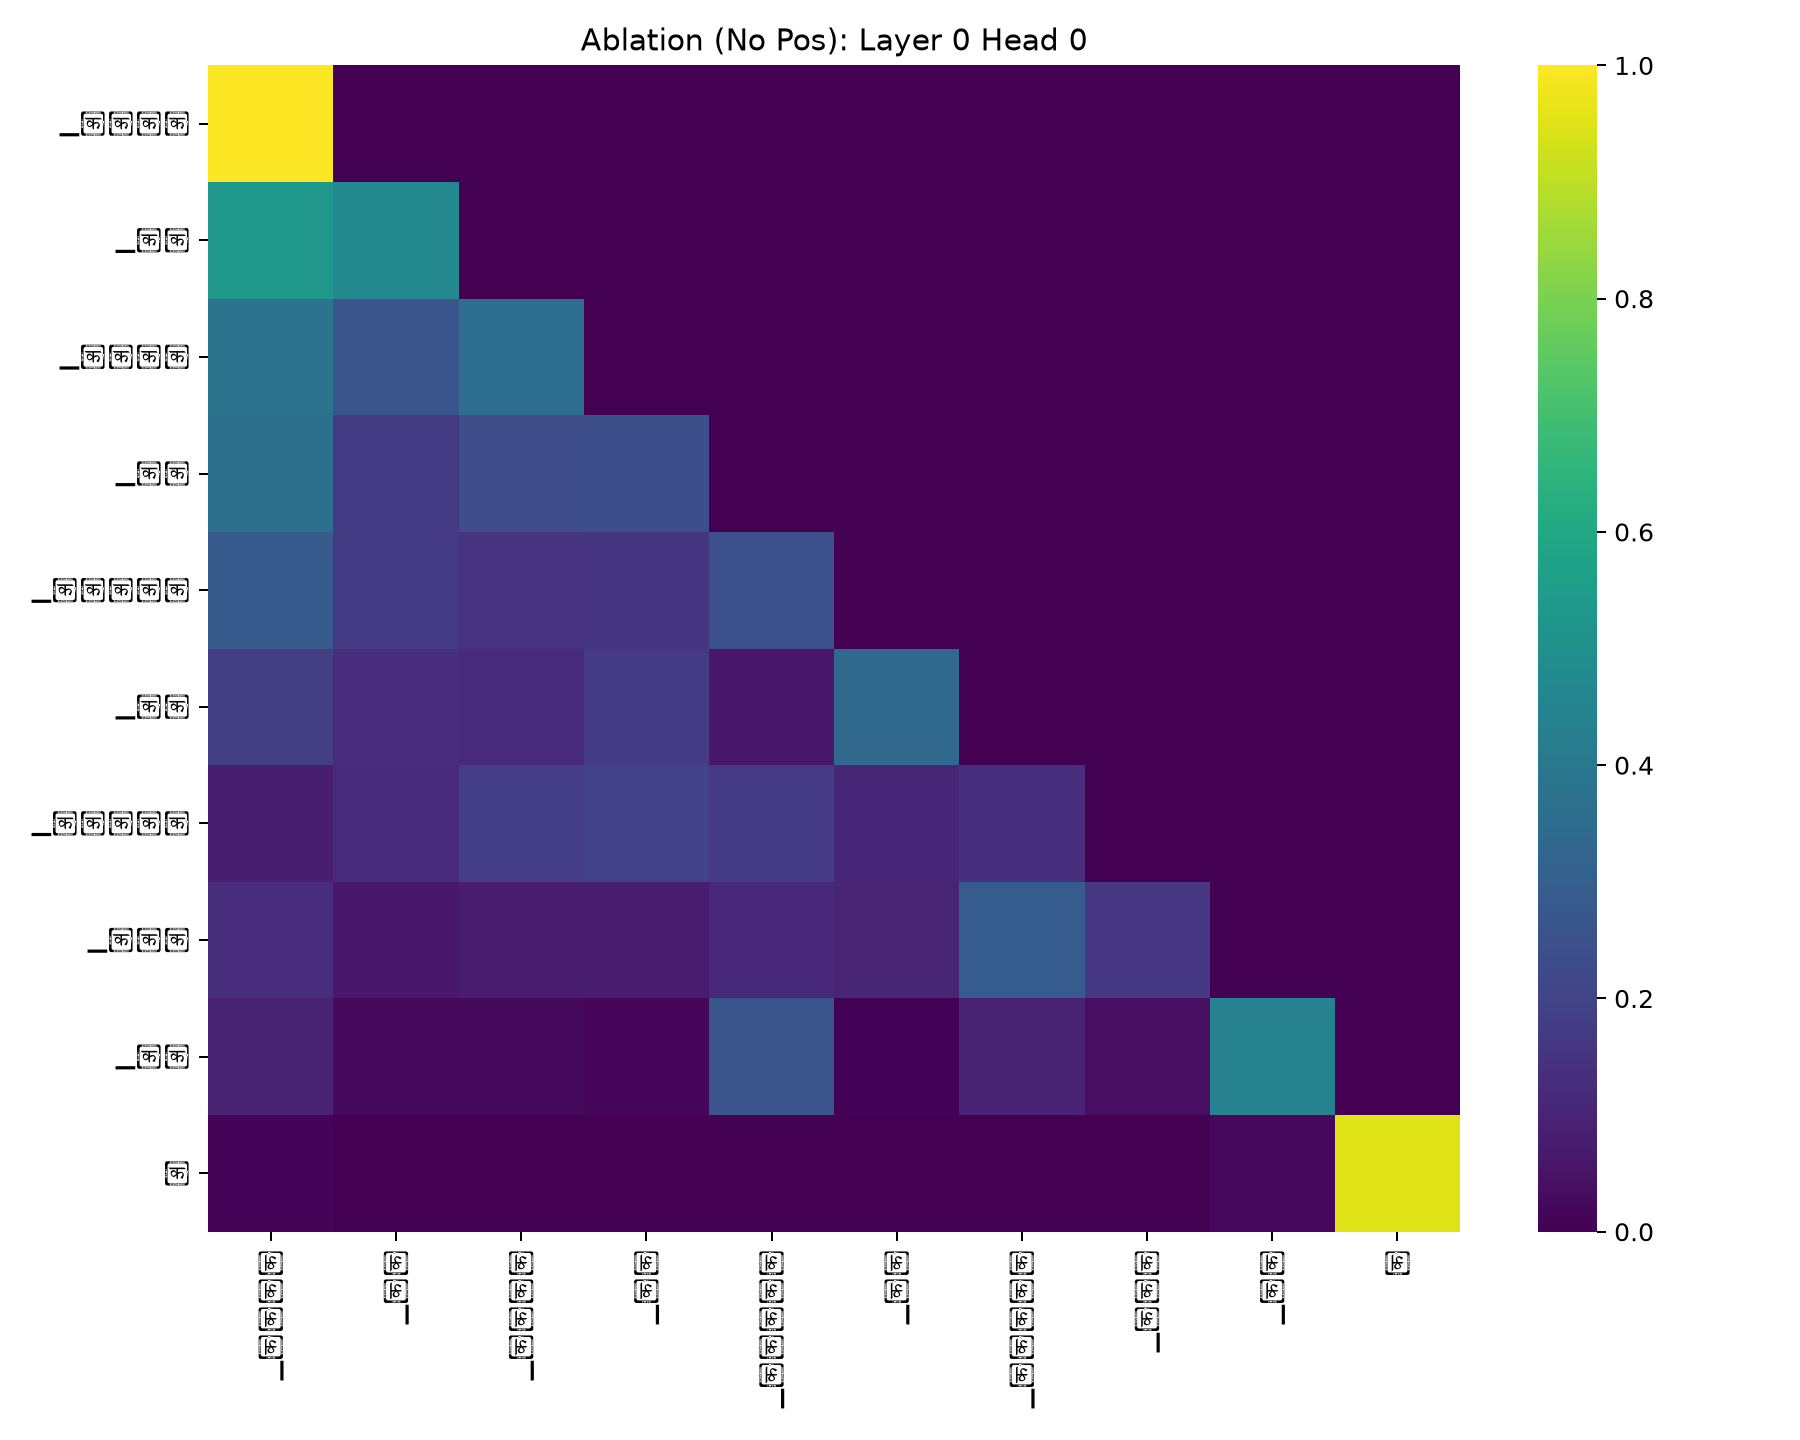
\includegraphics[width=\textwidth]{images/attn_L0_H0_no_pos.png}
    \caption{Ablated L0 H0}
\end{subfigure}
\hfill
\begin{subfigure}[b]{0.48\columnwidth}
    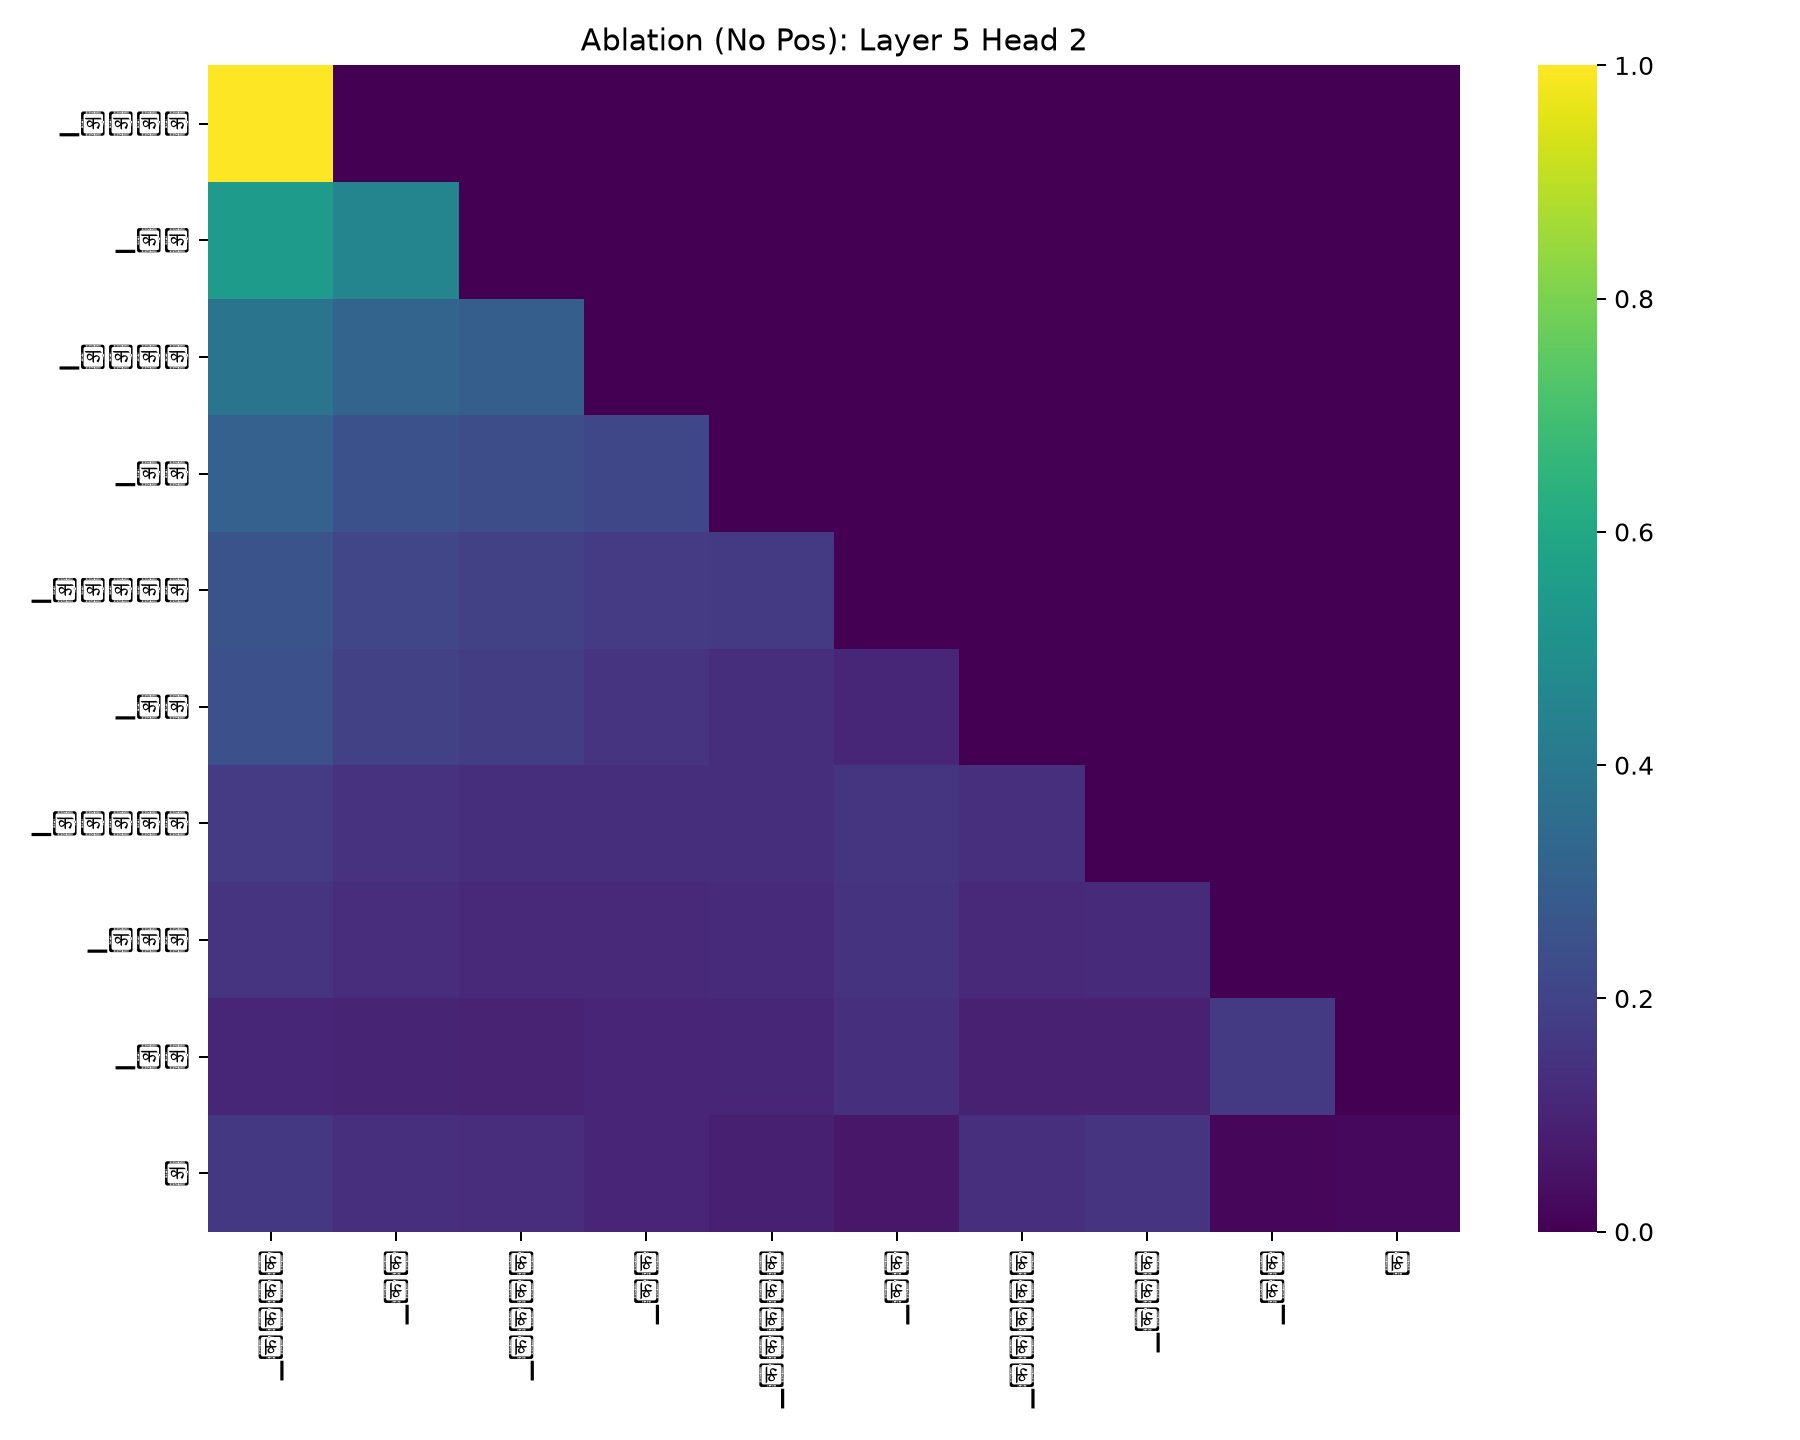
\includegraphics[width=\textwidth]{images/attn_L5_H2_no_pos.png}
    \caption{Ablated L5 H2}
\end{subfigure}
\caption{Ablated attention heatmaps showing loss of diagonal banding.}
\label{fig:bonus_attn}
\end{figure}

\subsection{What Breaks Without Position Information?}
\begin{enumerate}[noitemsep,leftmargin=*]
    \item \textbf{Syntax and Case-Role Inversion:} In Hindi SOV syntax, role assignment depends strictly on postposition word order (\textit{Ram ne Ravan ko mara} vs. \textit{Ravan ne Ram ko mara}). Without position, self-attention cannot bind nouns to their following postpositions, reducing sentential syntax to an unordered bag of words.
    \item \textbf{Autoregressive Attractor Loops:} Generation collapses into repeating high-frequency postpositions (\textit{"ke mein ke mein..."}). Without positional signals, the hidden state at step $t+1$ is structurally identical to step $t$, trapping the sampler.
    \item \textbf{Destruction of Long-Range Dependency Heads:} Layer 5 attention distance collapsed from \textbf{7.42 to 2.54 tokens}, destroying syntactic dependency tracking.
\end{enumerate}

\section{Authentic Student Reflections and Viva Defense Guide}

\subsection{Conceptual Principles Tested in Evaluations}
\begin{enumerate}[noitemsep,leftmargin=*]
    \item \textbf{Why Attention Requires $1/\sqrt{d_k}$ Scaling:} In high dimensions $d_k$, if components of $q$ and $k$ are independent random variables with zero mean and unit variance, their dot product $q^T k = \sum_{i=1}^{d_k} q_i k_i$ has mean 0 and variance $d_k$. As $d_k$ grows (here $d_k=64$), dot products become very large in magnitude, pushing the softmax into regions with extremely small gradients. Dividing by $\sqrt{d_k}$ restores unit variance, stabilizing backpropagation.
    \item \textbf{Why Upper Triangular Matrix is Masked and Set to Zero:} In causal auto-regressive generation, token $i$ must not attend to future tokens $j > i$. This is implemented by adding an upper-triangular matrix $M$ where $M_{ij} = -\infty$ for $j > i$ to the logits prior to softmax. Since $\exp(-\infty) = 0$, the post-softmax probabilities $A_{ij}$ in the upper triangle evaluate to strictly $0.0$, producing the characteristic dark purple region in all our heatmaps.
    \item \textbf{The Relation Between Cross-Entropy, Perplexity, and Bits-Per-Byte:} Cross-entropy loss $\mathcal{L} = -\frac{1}{N} \sum_{i=1}^N \ln P(w_i | w_{<i})$. Perplexity is the exponentiated loss $\text{PPL} = \exp(\mathcal{L})$, representing the effective branching factor. Bits-Per-Byte ($\text{BPB} = \frac{\mathcal{L}}{\ln 2} \times \frac{N_{\text{tokens}}}{N_{\text{bytes}}}$) measures compression efficiency independent of vocabulary size.
    \item \textbf{Why Attention Sinks Form Naturally:} The softmax function enforces a strict sum-to-one constraint: $\sum_{j=0}^{i} A_{ij} = 1.0$. In deep layers, when an attention head has no relevant syntactic dependency for the current query token, it must still allocate 100\% of its probability mass. The network naturally learns to designate the initial token (position 0) as an attention sink---a harmless dumping ground for unneeded attention weights that acts as a computational no-op valve.
\end{enumerate}

\subsection{Empirical Lessons and Engineering Realities}
\begin{enumerate}[noitemsep,leftmargin=*]
    \item \textbf{The PPL vs. Reasoning Paradox:} Low perplexity is an insufficient indicator of intelligence. Nepali achieved superior PPL (37.7 vs. 55.5) and BPB (5.24 vs. 5.79) during pretraining, yet its zero-shot reasoning was practically nonexistent (0.5\% vs. 12.0\%). High tokenizer fertility allowed the model to achieve low loss by predicting frequent subword morphemes without acquiring relational semantics.
    \item \textbf{Regularization in Small Transformers:} Training without Dropout enabled high hardware throughput but resulted in a 0.67 train-val loss gap in Hindi. In future iterations, implementing mild dropout ($p=0.1$) and LayerDrop would mitigate memorization.
    \item \textbf{Position Information is Indispensable:} The ablation study proved that Transformers do not possess inherent sequential awareness; without position encodings, perplexity explodes 47-fold and language modeling completely fails.
\end{enumerate}

\section{Master Deliverables and Artifact Index}

\begin{table}[H]
\centering
\footnotesize
\setlength{\tabcolsep}{2.5pt}
\caption{Master Index of Project Deliverables and Checkpoints}
\label{tab:deliverable_index}
\begin{tabularx}{\columnwidth}{@{}>{\raggedright\arraybackslash}p{2.3cm}>{\raggedright\arraybackslash}X@{}}
\toprule
\textbf{Deliverable} & \textbf{Resource / Drive Link / Repository Path} \\
\midrule
Phase 1 Code & \path{hindi/scripts/}, \path{nepali/scripts/} \\
Tokenizers & \path{hindi/tokenizer/}, \path{nepali/tokenizer/} \\
Phase 1 Splits & \href{https://drive.google.com/drive/folders/1WXVGFmtd4bqrctrEArb3Y-tlOfAA55dF?usp=sharing}{Hindi Splits} / \href{https://drive.google.com/drive/folders/1Lq7IYyVIRJTbLPG1fdc2if_RiI713HS7?usp=sharing}{Nepali Splits} \\
SQLite DBs & \href{https://drive.google.com/file/d/1EaZsr74aLL0g70TVOkbckQr62NDk90CH/view?usp=sharing}{Hindi DB (8GB)} / \href{https://drive.google.com/file/d/1avTD7KQ92QcKJojcmqSV3jb4bW1q3vHH/view?usp=sharing}{Nepali DB (11GB)} \\
\midrule
Phase 2 Code & \path{hindi/scripts/model.py}, \path{train.py}, \path{evaluate.py} \\
Pretrained Pts & \href{https://drive.google.com/file/d/1QpTcnaJEnypQP3c9NFM790h3enfT7xlm/view?usp=sharing}{Hindi final.pt} / \href{https://drive.google.com/file/d/1a7cVgfeJVn6-yiZWHhG2N4YwfBfJmdwh/view?usp=sharing}{Nepali final.pt} \\
Heatmap Code & \path{report/scripts/generate_all_head_heatmaps.py} \\
\midrule
Phase 3 Code & \path{phase3/scripts/generate_reasoning_data.py}, \path{finetune_reasoning.py} \\
Finetuned Pts & \href{https://drive.google.com/drive/folders/1SliWJWeMXxkpp7ybroLu3asjcFZnEQ7H?usp=sharing}{Hindi best.pt} / \href{https://drive.google.com/drive/folders/1JEJy1XVYIse2uOeSo7_7pW7SiMrnj-vo?usp=sharing}{Nepali best.pt} \\
Reasoning Data & \path{phase3/data/hindi/}, \path{phase3/data/nepali/} \\
\midrule
Ablation Code & \path{bonus/scripts/model_no_pos.py}, \path{train_no_pos.py} \\
Bonus Reports & \path{bonus/report.md}, \path{report/bonus_report.md} \\
Repository & \href{https://github.com/CL3-410/individual-project-Rajkjain03/tree/phase-3}{GitHub Repository (phase-3 branch)} \\
\bottomrule
\end{tabularx}
\end{table}

\end{document}
